%
%
%

\section{Top Quark Pair-Production Cross-Section Combination}

A precise measurement of the Top Quark Pair-Production Cross-Section is crucial for understanding the performance of the ATLAS detector, for testing predictions of the standard model, to searching for or constraining many new physical models.
In particle physics, a cross-section is a way to describe the rate of a specific interaction or class of interactions independently of beam conditions that are used to produce it.
The value of the top-quark pair-production cross-section in the Standard Model can be predicted using Monte-Carlo simulation techniques \cite{TOP_XSC_THEORY} \cite{TTBAR_HADRON_COLLIDERS} \cite{THRESHOLD_EXPANSION_XSC}.
This value can be determined using ``Next to Leading Order'' techniques (NLO) and is corrected by adding the ``Next to Next to Leading Order'' soft logarithm terms (approximate NNLO).
This value is determined to be $\sigma_{\ttbar} = 165^{11}_{16}$ with an uncertainty below 10\%.
The most accurate experimental determinations of the top quark's cross section previous to the LHC's results were measured by the CDS and the D0 collaborations at the Tevatron \cite{TEVATRON_XSC_LJETS} \cite{TEVATRON_XSC_DILEP}.
These experiments determined the cross-section at a center-of-mass energy of $\sqrt{s} = 7 TeV$ to a precision of 8\% using individual channels and 6.4\% by combining measurements across multiple channels.

The top-quark pair-production cross section has been measured at ATLAS using many channels and analysis technqiues.
The most precise measurements use combination of several individual measurements, which reduces both statistical and systematic uncertainties.
This section presents an ATLAS measurement of the $\ttbar$ cross-section that statistically combined three separate analysies strategies.
The likelihoods for measurements using single-lepton, dilepton, and all-hadronic channels were modeled as functions of the top cross-section, as well as a variety of nuisance parameters.
% This combination was performed by modeling the likelihoods of several individual measuremnets as functions of the top cross-section as well as a variety of nuisance parameters.
These likelihoods were then merged and a simultaneous fit to the measured data across all channels was performed.

The combined measurement of the $\ttbar$ cross-section used a measurement in the lepton+jets channel which was performed using 0.7$\ifb$ of data recorded in 2011 \cite{LEPTON_JETS_NOTE_2011}, a measurement in the dilepton channel which was performed using 0.7 $\ifb$ of data collected in 2011 \cite{DILEPTON_PAPER}, and a measurement in the all-hadronic channel, which was performed using 1.02 $\ifb$ of data collected in 2011 \cite{ALL_HADRONIC_NOTE}.


\subsection{Top Quark Pair-Production}

The primary means of producing top quarks at the LHC is via gluon fusion and subsequent decay into a pair of top quarks.

\begin{figure}
  \begin{center}

    \subfigure[Production]{
      % TopQuarkPairProductionDiagram: http://kjende.web.cern.ch/kjende/netzwerk/images/Feynman/WplusWminusBBar.png
      \includegraphics[width=.4\linewidth]{figures/xsection/TopQuarkPairProductionDiagram.png}
    }
    \subfigure[Decay]{
      % TopQuarkBranchingRatios: http://ej.iop.org/images/0034-4885/75/5/056201/Full/rpp347183f06_online.jpg
      \includegraphics[width=.4\linewidth]{figures/xsection/TopQuarkBranchingRatios.jpg}
    }
  \end{center}
  \caption{ A typical feynman diagram of top quark pair production at the LHC.  Top quarks decay into W-bosons and b-quarks nearly 100\% of the time.  The subsequent decays of the W-Bosons determine the event topology of the \ttbar event.  Diagram showing the branching ratios of Top Quark pairs into leptons and quarks.}
  \label{img:TopQuarkPairProduction}
\end{figure}

W bosons decay either leptonically, in which they produce a lepton and a neutrino, or hadronically, in which they produce a pair of quarks.
W's decay leptonically 32.6\% of the time, which consists of decaying via $W- \rightarrow e \bar{\nu_{e}}$ 10.75\% of the time, via $W- \rightarrow \mu \bar{\nu_{\mu}}$ 10.57\% of the time, and via $W- \rightarrow \tau \bar{\nu_{\tau}}$ 11.25\% of the time, and decay into quarks the other 67.60\% of the time. \cite{PARTICLE_DATA_GROUP}
% W-Boson: http://pdg.lbl.gov/2012/listings/rpp2012-list-w-boson.pdf
However, tau leptons are themselves unstable particles that subsequently decay either leptonically (muon 17.41 or electron 17.83), or hadronically 64.76\% of the time, with about 50\% of the tau's today decays into 1 hadron and 15\% into 3 hadrons.
% Tau pdg: http://pdg.web.cern.ch/pdg/2012/listings/rpp2012-list-tau.pdf
In the discussion that follows, leptonic decays of a top quark include $t \rightarrow W \rightarrow \tau \rightarrow e$ or $t \rightarrow W \rightarrow \tau \rightarrow \mu$, and we will ignore the intermediate state $\tau$ in terms of our classification.
Hence, a pair of top quarks, which we assume always decay into a pair of W bosons, will decay into two leptons 6.5\% of the time (known as the ``dilepton'' channel), into a single lepton and a pair of quarks 34.4\% of the time (known as the ``single lepton'' channel), and entirely into quarks 45.7\% of the time (known as the ``all hadronic'' channel).
% pdg:
% Citation: J. Beringer et al. (Particle Data Group), PR D86, 010001 (2012) (URL: http://pdg.lbl.gov)



%% \begin{figure}
%%   \begin{center}
%%     % TopQuarkBranchingRatios: http://ej.iop.org/images/0034-4885/75/5/056201/Full/rpp347183f06_online.jpg
%%     \includegraphics[width=100mm]{figures/xsection/TopQuarkBranchingRatios.jpg}
%%   \end{center}
%%   \caption{}
%%   \label{img:TopQuarkBranchingRatios}
%% \end{figure}

\subsection{Object Reconstruction}

Measurements of $\ttbar$ event require kinematicaly reconstructing and selecting a variety of physical objects, including electrons, muons, jets, b-jets, and $\MET$.

% Selected Electrons
Selected electrons are required to have a calorimeter cluster located in a pseudorapidity range of $0 < |\eta| < 4.47$, excluding the range $1.37 < |\eta| < 1.52$ (this excluded interval, known as the crack region, is a mostly un-insturmented part of the EM calorimeter).
To reject jets that fake electrons, the electron's energy is required to be isolated in the calorimeter.
Specifically, electrons with more than 3.5 GeV of energy in a cone of $\sqrt{(\Delta \eta)^2 + (\Delta \phi)^2}$, excluding the energy of the electron itself, are rejected.
Electrons must pass a variety of cuts related to the shape of its shower and the quality of its corresponding track that are collectively referred to as ``tight'' EM identification cuts.
Finally, Electrons must have a minimum energy of $E_{T} > 20$ GeV, where $E_{T}$ referrs to the transverse energy of the electron's electromagnetic cluster..

%% The selection of l + jets tt ̄ events makes use of reconstructed electrons, muons and jets, and the transverse momentum imbalance referred to as missing transverse energy Emiss.
%% T Electron candidates are reconstructed from the energy depositions in the electromagnetic calorimeter
%% and are required to have a well-measured track associated with the electromagnetic cluster. The latter is required to have |ηcluster| < 2.47 excluding 1.37 < |ηcluster| < 1.52 corresponding to the transition region between barrel and endcap calorimeters. To ensure that electrons are isolated from the jet activity, as expected for prompt electrons from W boson decay, the energy in a cone of ∆R ≡ 􏰮∆η2 + ∆φ2 = 0.2, centered around the electron, excluding the energy associated with the electron itself, is required to be < 3.5 GeV. This defines the tight electron candidates used for the final analysis. Loose electron candidates employed for the estimation of the QCD multijet background, as described in Section 4, have to fulfill less stringent requirements and the isolation cut is increased to < 6 GeV energy deposition in ∆R = 0.2.

% Selected Muons
Selected Muons must be ``combined'', meaning they must use tracks from both the muon spectrometer and the inner detector.
Only muons within $|\eta| < 2.5$ are considered, and muons within $\Delta R <= 0.4$ of a selected jet are rejected.
Two isolation requirements are imposed on selected muons.  
They must be isolated in the calorimeter, meaning the energy deposited in the calorimeter within $\Delta R = 0.3$ must be $<$ 4 GeV, and their tracks must be isolated, meaning the sum of the transverse momenta of tracks in a code of $\Delta R = 0.3$ surronding the muon's track must be $<$ 4 GeV.

%% Muon candidates are reconstructed by searching for track segments in the different layers of the muon spectrometer. These segments are then combined starting from the outermost layer, and matched with the inner detector tracks. The final parameters of muon candidates are obtained from the combined fit using information from both detector systems. Only muons within |η| < 2.5 are included in this measurement. Like electrons, muons are required to be isolated, i.e. (i) be separated from the closest jet by ∆R(μ, jet) > 0.4; (ii) have calorimeter isolation < 4 GeV and (iii) have track isolation < 4 GeV. Track isolation is defined as the sum of track transverse momenta in a cone ∆R ≡ 􏰮∆η2 + ∆φ2 = 0.3, excluding the pT of the muon track, while calorimeter isolation is defined as energy deposition in the calorimeter within a cone of ∆R = 0.3, excluding the energy deposition directly along the muon track. Muons passing all requirements are used in the analysis sample selection and are referred to as tight, while muons with a looser isolation are used for the QCD multijet background estimate described in Section 4. In this case, all requirements except the cuts on calorimeter and track isolation have to be fulfilled and the muons are referred to as loose.

% Selected Jets
In this analysis, Jets are constructed using the anti-kt algorithm with a distance parameter of $R=0.4$.
These jets are built out of ``topoligical clusters'', which themselves are collections of neighboring cells that each have an energy above some threshold, where the energy has been calibrated to the scale of electromagnetic showers (known as ``Electromagnetic Scale'').
Once the jets are built, their energies are then recalibrated to the scale of hadronic particles (known as the ``Hadronic scale'') \cite{JES_SCALE_2010}.
Since jets are built out of calorimeter deposits, essentially all electrons will also be reconstructed as jets.
Therefore, these objects must be removed from the collection of selected jets by-hand.
In this analysis, any jet that overlaps with a selected electron within $\Delta R < 0.2$ is removed.

%% Jets are reconstructed using the anti-kt algorithm with distance parameter R = 0.4 [9] which sets the relative distance at which jets are resolved from each other. As input, the algorithm uses topological clusters that group together neighboring calorimeter cells with energy deposits above certain thresholds. Their energy accounts correctly for the energy deposited in the calorimeter by electromagnetic showers. Additional correction factors dependent on jet η and pT are applied to the reconstructed jets to correct their energy to the hadronic scale. The jet energy scale (JES) is established using corrections derived from collision and test beam data and calibration constants obtained from MC simulation [10]. Since reconstructed electrons might also be reconstructed as jets in the calorimeter, any jet overlapping with a %% 2 %% tight electron within a cone of ∆R < 0.2 is removed from the list of jets. 

%% MET
Finally, once all objects have been selected, the $\MET$ is defined as the vector sum of the calorimeter energy deposits of selected objects or the combined energy for muons (including additional corrections for energy deposited in the calorimeter).
The energy associated with each object is calibrated to the scale of that object, and all remaining energy deposits are added to the $\MET$ vector, but at electromagnetic scale.

%% The analysis reconstructs the missing transverse energy from the vector sum of energy depositions
%% in the calorimeter in the transverse plane associated to the objects used in the analysis. The same recon-
%% struction and identification algorithms as for the analysis objects are used to identify electrons and jets.
%% The corresponding topological clusters in the calorimeters are then included in the calculation of Emiss at T
%% the energy scale of the associated object. The muon momenta are calculated using the information from both the inner detector and the muon spectrometer system and corrected for additional energy deposi- tion in the calorimeter. Remaining energy depositions not associated to any object are included at the electromagnetic energy scale.

%% END

\subsection{Lepton+Jets}
The lepton$+$jets channel is the most statistically powerful decay of the $\ttbar$ system for measuring the pair-production cross-section.
The leptonic decay of one of the top results in an event topologiy that allows for strong background discrimination, while the hadronic decay of the other top maintains a high branching ratio for this channel.
The distinguishing features of the lepton$+$jets channel is the presence of a high-pt lepton from the leptonic decay of a W boson,v$\MET$ from a neutrino, two b-jets from the decay $t \rightarrow W+b$, and two additional jets from the hadronic decay of a W boson.
This topology of event was selected for by first requiring a single lepton trigger, which either required an electron or a muon (reconstructed by the trigger) with $E_{T} > 20 GeV$ or $p_{T} > 18 GeV$, respectively.
The exact trigger required varied throught the run periods of 2011 as higher instintaneous luminosities required stricter lepton definitions to maintain a steady bandwidth of recorded events as selected by the trigger.
Selected events are required to have a primary vertex that consists of 5 or more tracks.
Each event must have exactly 1 selected electron or muon, and that lepton must match a corresponding object that fired a single-lepton trigger (events with more than 1 lepton fall into the dilepton channel, to be described in detail later).
The energy requirements for these objects were chosen to minimize any effects resulting from the trigger's online reconstruction.
A cut on $\MET$ is imposed, requiring $\MET > 35 GeV$ for the electron channel and $\MET > 25 GeV$ for the muon channel (the difference in the cut results from different background contributions to each channel from QCD events, which tend to have low values of $\MET$).
Additional cuts are made on the to reduce the contamination from QCD, which use a variable known as the ``W boson transverse mass'':
\begin{equation}
  m_{T}(W) = \sqrt(2 p_{T}^{l} p_{T}^{\nu} (1 - cos( \phi^{l} - \phi^{\nu}))),
\end{equation} 
where the $\MET$ vector is used to determine the kinematic variables of the neutrino, $p_{T}^{\nu}$ and $\phi^{\nu}$.
Using this definition, the event selection requires $m_{T}(W) > 25 GeV$ in the electron channel or $\MET + m_{T}(W) > 60 GeV$ in the muon channel.



\subsubsection{Backgrounds}
A selection of events based on the above criteria will be contaminated with several sources of backgrounds, including

\begin{itemize}
\item QCD Multijet events where a lepton is faked via a background mechanism
\item $W+Jets$ events where the W decays leptonically (leading to $\MET$) which includes real or fake b-jets
\item $Z+Jets$ events where one of the two leptons isn't identified and which includes real or fake b-jets
\item Diboson Events (WW, WZ, or ZZ events), that include some combination of leptonic decays of vector bosons, additional jets, and real or faked b-jets
\item Single Top events
\end{itemize}

% Add figures

\begin{figure}
  \begin{center}
    \subfigure[$W+Jets$]{
      % 
      \includegraphics[width=.4\linewidth]{figures/xsection/ZJetsDiagram.png}
    }
    \subfigure[$QCD$]{
      %ZJetsDiagram.png : http://inspirehep.net/record/871058/files/qg_qZ.png
      \includegraphics[width=.4\linewidth]{figures/xsection/ZJetsDiagram.png}
    } \\
    \subfigure[$Z+Jets$]{
      %ZJetsDiagram.png : http://inspirehep.net/record/871058/files/qg_qZ.png
      \includegraphics[width=.4\linewidth]{figures/xsection/ZJetsDiagram.png}
    }
    \subfigure[$Single Top$]{
      % 
      \includegraphics[width=.4\linewidth]{figures/xsection/ZJetsDiagram.png}
    } \\
  \end{center}
  \caption{Feynman diagrams for the most important backgrounds to $\ttbar$ events.  Shown are $Z+Jets$ events (top, left), $W+jets$ events (top, right), QCD events (bottom, left) and Single Top events (bottom, right).}
  \label{img:BackgroundsFeynmanDiagrams}
\end{figure}

To measure the cross-section, the background contributions due to each of the above processes in the lepton+jets channel were determined using a variety of techniques.
The dominant $W+Jets$ background as well as the $Z+Jets$, diboson, and single-top background are estimated using Monte-Carlo simulation.
While the kinematic distributions of each $W+Jets$ event were estimated from Monte-Carlo, the expected number of events was extracted using a data-driven technique.
The technique used to estimate the normalization of the $W+Jets$ background is based on one used in a top-quark charge-asymmetry analysis \cite{CHARGE_ASYMMETRY}.
It is based on the fact that $W^{+}$ bosons are produced at a higher rate than $W^{-}$ bosons due to the fact that the LHC collides protons (and not anti-protons).
The ratio of the production of $W^{+}$ to $W^{-}$, $r_{MC}$, can be estimated using Monte-Carlo.  Assuming that $W+Jets$ events are the dominant category of events that are asymmetric between positive and negative leptons, one can estimate the total number of $W+Jets$ events by taking the difference between the measured jumber of events with a positive lepton and the number with a negative lepton:

\begin{equation}
  N_{W^{+}} + N_{W^{-}} = \frac{r_{MC} + 1}{r_{MC} - 1}(D^{+} - D^{-}),
\end{equation}

where $D^{+}$ and $D^{-}$ are the number of selected single-lepton events with a positive or negative lepton, respectively.
The value of $r_{MC}$ is measured to be 1.56 $\pm$ 0.07 for the electron channel and 1.66 $\pm$ 0.06 for the muon channel.
Estimates of overall yields or kinematic variables for the $W+Jets$ background are then weighted to a total normalization given by this data-driven value.
The normalizations for the $Z+Jets$, diboson, and single-top backgrounds are taken directly from cross-sections evaluated using monte-carlo and scaled to the integrated luminosity recorded by the ATLAS detector.

Each of the backgrounds which are estimated using Monte-Carlo lead to real leptons in the final state.
In contrast, the QCD background enters the single-lepton channel when a final state jet is falsely identified as a lepton.
The process of a jet faking a lepton depends on the details of the jet's hadronic shower, in particular it's shape and depth in both the electromagnetic and hadronic calorimeters.
The hadronic shower evolution is of course modeled in detail by simulations used by ATLAS.
However, small differences in the nature of that simulation can lead to significant changes in the rate of jets faking leptons.
And because the number of QCD events created at ATLAS is extremely large, changes in the rate will have dramatic differences in the number of background events in the lepton+jets signal region.
For this reason, it is preferable to estimate the background contribution due to QCD without relying on the details of the Monte-Carlo description of hadronic shower evolution.

The lepton+jets analysis uses a technique to extract the rate and distribution of QCD events from data directly.
Known as the ``Matrix Method,'' this technique exploits the fact that the efficiencies of real and fake leptons differ as a function of cuts on the reconstructed lepton's isolation and shower shape.
The technique involves creating two subsets of lepton identifications, denoted as ``loose'' and ``tight'' (with ``tight'' corresponding to the nominal selection requirements).
The Matrix Method relies on knowing the effecienciy for both real and fake leptons which pass loose selection to also pass the tight selection.

\begin{equation}
  \epsilon_{real} = \frac{N^{tight}_{real}}{N^{loose}_{real}} and \epsilon_{fake} = \frac{N^{tight}_{fake}}{N^{loose}_{fake}},
\end{equation}

where $N^{tight}$ and $N^{loose}$ represent the number of events with tight or loose (and not tight) lepton, respectively, in the region of phase space where the efficiency is being measured.
Given these values, one can write a set of equations relating the number of events with a measured loose or tight lepton to the number  

\begin{eqnarray}
  \bar{N^{tight}} = \epsilon_{real} N_{real} + \epsilon_{fake} N_{fake} \\
  \bar{N^{loose}} = (1-\epsilon_{real}) N_{real} + (1-\epsilon_{fake}) N_{fake}.
  \label{eq:MatrixMethod}
\end{eqnarray}

The above equations can be inverted to obtain $N_{fake}$ and $N_{real}$, quantities we're interested in estimating, as a function of  $N^{tight}$ and $N^{loose}$, quantities that can be measured.
By solving and isolating the variables $N^{tight}_{real}$ and $N^{tight}_{fake}$ (which represent the real and fake lepton contributions to the tight, or signal, region), and expressing the solution as a matrix, we obtain the following:

\begin{eqnarray}
  N^{tight}_{real} = \frac{N^{tight} - \epsilon_{fake}N^{loose}}{\epsilon_{fake} - \epsilon_{real}} \\
  N^{tight}_{fake} = \frac{\epsilon_{real}N^{loose} - N^{tight}}{\epsilon_{fake} - \epsilon_{real}}
\end{eqnarray}

\begin{equation}
\begin{pmatrix} N^{tight}_{real} \\ N^{tight}_{fake} \\ \end{pmatrix} 
  = 
  \begin{pmatrix} 
    \frac{\epsilon_{real}}{\epsilon_{real} - \epsilon_{fake}} & \frac{-\epsilon_{real}\epsilon_{fake}}{\epsilon_{real} - \epsilon_{fake}} \\ 
    \frac{-\epsilon_{fake}}{\epsilon_{real} - \epsilon_{fake}} & \frac{\epsilon_{real}\epsilon_{fake}}{\epsilon_{real} - \epsilon_{fake}} \\ 
  \end{pmatrix}  
  \begin{pmatrix} N^{tight} \\ N^{loose} \\ \end{pmatrix}
  \label{eq:MatrixMethodInverted}
\end{equation}

One should note that the solution is linear in the number of tight or loose events.
In particular, this means that we can associate any given event (be it loose or tight) with a weight for real or fake, and these weights are simply the (1,1) and (2,1) elements of the matrix in equation \ref{eq:MatrixMethodInverted}.
Therefore, in the case that the $\epsilon$ values are functions of arbitrary variables associated with an event, one can still estimate the number of fakes in the tight (signal) region as:

\begin{equation}
  N^{tight}_{fake} = \sum_{e \in tight} (\frac{-\epsilon_{fake}}{\epsilon_{real} - \epsilon_{fake}}) + \sum_{e \in loose} (\frac{\epsilon_{real}\epsilon_{fake}}{\epsilon_{real} - \epsilon_{fake}})
  \label{eq:MatrixMethodSum}
\end{equation}

Equation \ref{eq:MatrixMethodSum} is used to estimate the amount of QCD multijet events that enter the signal region (assuming that all fakes in the loose or tight regions come from QCD Multijet events).
In that estimation, loose electrons are defined identically as tight electrons, except their isolation cut is relaxed, requiring that $E_{T} < 6 GeV$ in a cone defined by $\Delta R = 0.2$.
Similarly, loose muons are identical to tight muons, but the cuts on $E_{T}$ and $p_{T}$ isolation are removed entirely.
The efficiencies for loose leptons, as defined above, to also pass tight requirements for both real and fake muons are measured directly in data.
To measure the efficiencies of real leptons, a collection of events dominated by $Z->ee$ or $Z->\mu\mu$ is created by selecting dilepton events where the invariant mass of the leptons is close to the mass of the Z-boson.
In such a sample, the efficiency can be measured directly.
For fake leptons, a sample of QCD multijet events is collected by selecting events with a single (loose) lepton, a jet, and by requiring $5 GeV < \MET <  60 GeV$ for electron events or $m_{T}(W) < 20 GeV$ and $m_{T}(W) + \MET < 60 GeV$ for muon events.
For muons, the efficiencies were paramaterized as a function of the muon's $p_{T}$ and $\eta$.
Contributions from $Z+Jets$ and $W+Jets$ in the QCD control regions were subtracted using Monte-Carlo estimates.

% e + Jets
\begin{table}
  \begin{tabular}{lccccc}
    \hline
    $e + Jets$ & 1 Jet & 2 Jet & 3 Jet & 4 Jet & $>=$ 5 Jets \\ 
    \hline
    $\ttbar$ & $225 \pm 15$ & $1005 \pm 32$ & $1934 \pm 44$ & $1835 \pm 43$ & $1463 \pm 38$ \\
    $W+Jets$ & $161600 \pm 400$ & $43170 \pm 210$ & $10840 \pm 100$ & $2486 \pm 50$ & $1032 \pm 32$ \\
    $QCD Multijets$ & $11000 \pm 5000$ & $4800 \pm 2400$ & $1600 \pm 800$ & $510 \pm 250$ & $117 \pm 89$ \\
    Single Top & $571 \pm 24$ & $711 \pm 27$ & $391 \pm 20$ & $156 \pm 13$ & $65 \pm 8$ \\
    $ZJets$ & $3732 \pm 61$ & $2444 \pm 49$ & $996 \pm 32$ & $333 \pm 18$ & $146 \pm 12$ \\
    Diboson & $599 \pm 25$ & $538 \pm 23$ & $178 \pm 13$ & $45 \pm 7$ & $10 \pm 3$ \\
    \hline
    Total Predicted & $177000 \pm 5000$ & $52600 \pm 2400$ & $15900 \pm 800$ & $5360 \pm 260$ & $2892 \pm 100$ \\
    Total Observed & 179469 & 51820 & 15614 & 5398 & 2812 \\
    \hline
  \end{tabular}
  \caption{Predicted and observed event yields in bins of jet number for the $\ttbar$ signal and backgrounds in the $e+jets$ channel.  Yields are obtained using Monte Carlo or Data-Driven techniques, depending on the sample.}
\end{table}

% mu + Jets
\begin{table}
  \begin{tabular}{lccccc}
    \hline
    $e + Jets$ & 1 Jet & 2 Jet & 3 Jet & 4 Jet & $>=$ 5 Jets \\ 
    \hline
    $\ttbar$ & $319 \pm 18$ & $1342 \pm 37$ & $2734 \pm 52$ & $2714 \pm 52$ & $2030 \pm 45$ \\
    $W+Jets$ & $383200 \pm 600$ & $93440 \pm 310$ & $20140 \pm 140$ & $4644 \pm 68$ & $1082 \pm 33$ \\
    $QCD Multijets$ & $25000 \pm 12000$ & $11000 \pm 6000$ & $3200 \pm 1600$ & $900 \pm 400$ & $290 \pm 150$ \\
    Single Top & $996 \pm 32$ & $1148 \pm 34$ & $594 \pm 24$ & $210 \pm 15$ & $84 \pm 9$ \\
    $ZJets$ & $17270 \pm 130$ & $5492 \pm 74$ & $1510 \pm 39$ & $436 \pm 21$ & $149 \pm 12$ \\
    Diboson & $1093 \pm 33$ & $1009 \pm 32$ & $308 \pm 18$ & $69 \pm 8$ & $18 \pm 4$ \\
    \hline
    Total Predicted & $428000 \pm 12000$ & $113000 \pm 6000$ & $28400 \pm 1600$ & $8900 \pm 400$ & $3660 \pm 160$ \\
    Total Observed & 433931 & 111741 & 28643 & 8680 & 3814 \\
    \hline
  \end{tabular}
  \caption{Predicted and observed event yields in bins of jet number for the $\ttbar$ signal and backgrounds in the $\mu+jets$ channel.  Yields are obtained using Monte Carlo or Data-Driven techniques, depending on the sample.}
\end{table}


\begin{figure}
  \begin{center}
    \subfigure[$e+jets$] {
      % EJetsYieldPlot.eps: https://atlas.web.cern.ch/Atlas/GROUPS/PHYSICS/CONFNOTES/ATLAS-CONF-2011-121/fig_01a.eps
      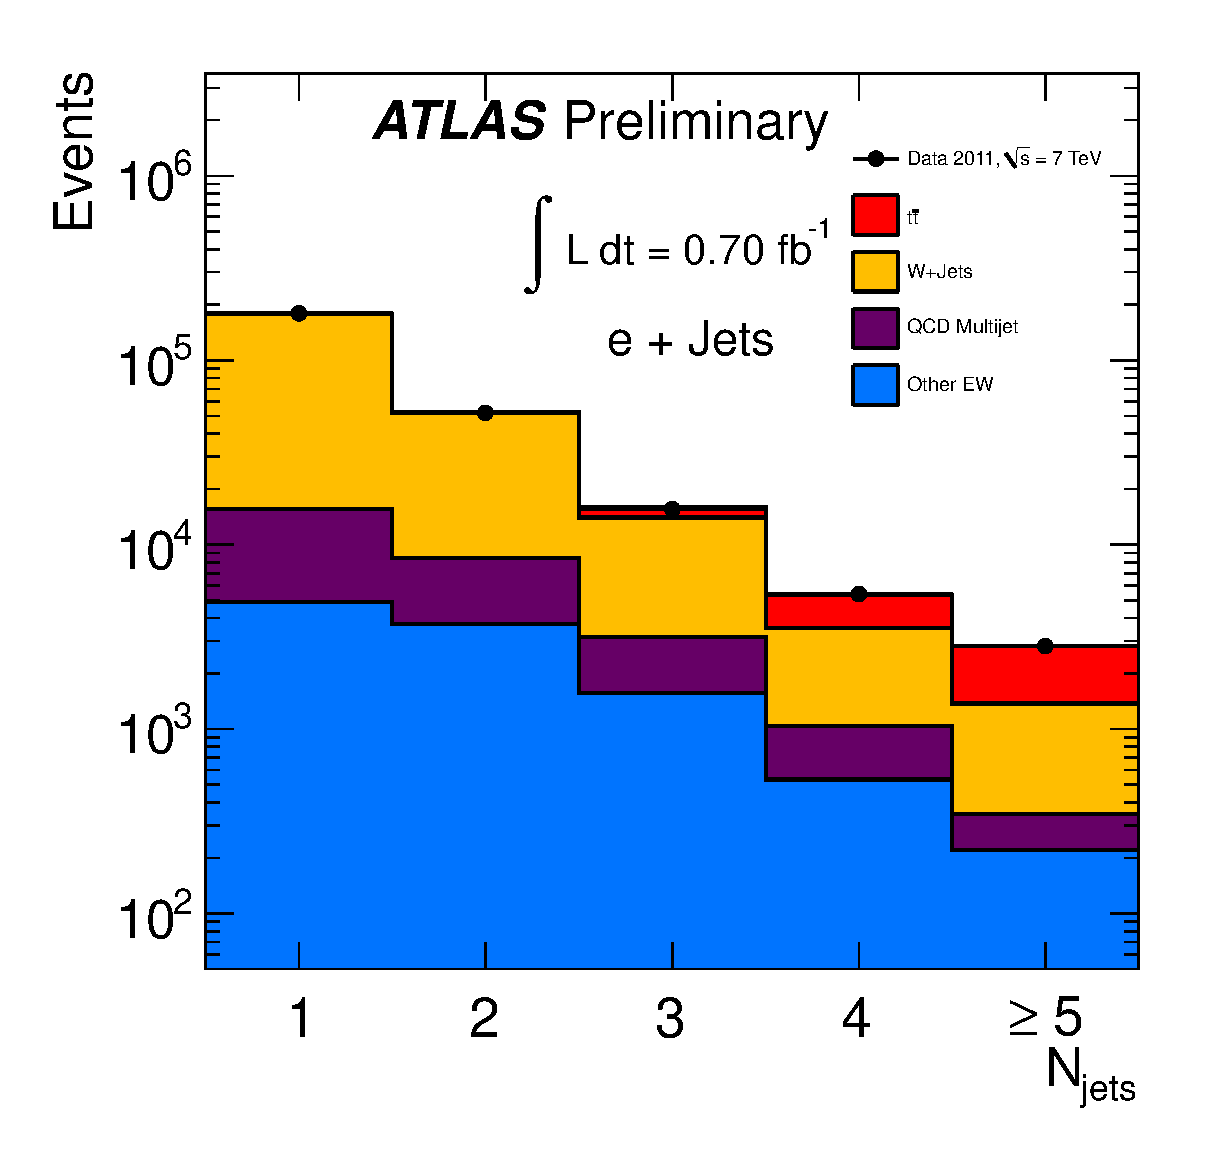
\includegraphics[width=.45\linewidth]{figures/xsection/EJetsYieldPlot}
    }
    \subfigure[$\mu+Jets$] {
      % MuJetsYieldPlots.eps: https://atlas.web.cern.ch/Atlas/GROUPS/PHYSICS/CONFNOTES/ATLAS-CONF-2011-121/fig_01b.eps
      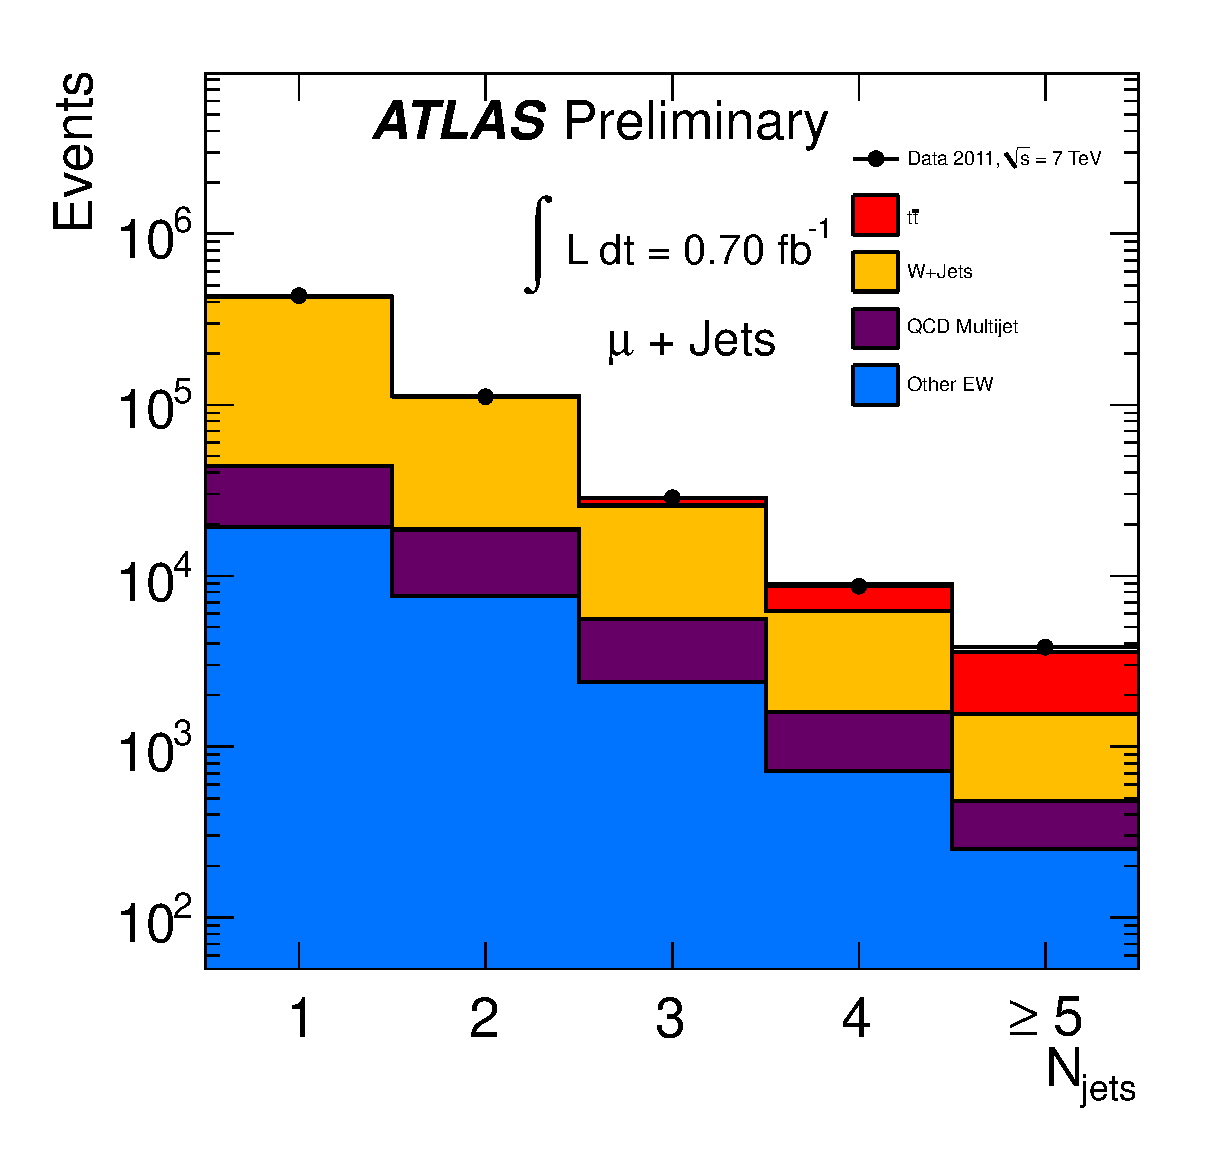
\includegraphics[width=.45\linewidth]{figures/xsection/MuJetsYieldPlot} %  figures/xsection/MuJetsYieldPlots}
    }
  \end{center}
  \caption{The yields of signal and backgrounds in bins of jet number.}
  \label{img:JetNumberYieldPlots}
\end{figure}


% https://atlas.web.cern.ch/Atlas/GROUPS/PHYSICS/CONFNOTES/ATLAS-CONF-2011-121/fig_01a.eps
% https://atlas.web.cern.ch/Atlas/GROUPS/PHYSICS/CONFNOTES/ATLAS-CONF-2011-121/fig_01b.eps


The measurement of the $\ttbar$ cross-section is obtained by fitting multiple multivariate distributions to measured data simultaneously.
These distributions are built out of four kinematic variables: the pseudorapidity of the selected lepton, the $p_{T}$ of the jet with the highest $p_{T}$, the event aplanrity and a variable denoted as $H_{T,3p}$.
The aplanarity, $A$, is defined as 1.5 times the smallest eivenvalue of the matrix

\begin{equation}
  M_{i,j} = \frac{ \sum_{k=1}^{N'_{objects}} p_{ik}p_{jk} }{ \sum_{k=1}^{N'_{objects}} p_{k}^2 }
  \label{eq:Aplanarity}
\end{equation}

and $H_{T, 3p}$, which is the total transverse momentum of all jets except for the first two normalized to the longitudinal momenta of all objects, is given by:

\begin{equation}
  H_{T, 3p} = \frac{ \sum_{i=3}^{N_{jets}} |p_{T, i}| }{ \sum_{j=1}^{N_{objects}} |p_{Z,j}|  }
\end{equation}


\begin{figure}
  \begin{center}
    \subfigure[leading jet $p_{T}$] {
      % DiscrimPtjet4Jets: https://atlas.web.cern.ch/Atlas/GROUPS/PHYSICS/CONFNOTES/ATLAS-CONF-2011-121/fig_04c.eps
      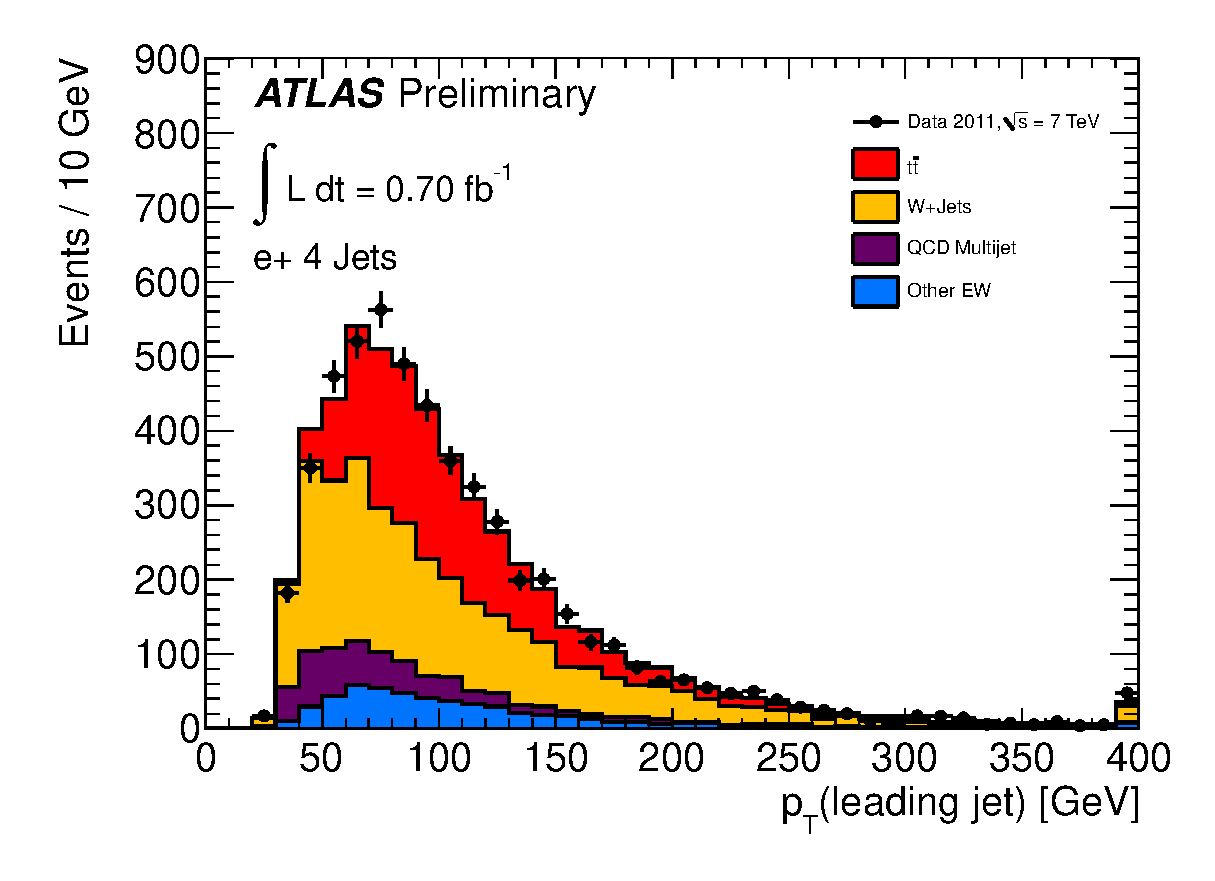
\includegraphics[width=.45\linewidth]{figures/xsection/DiscrimPtjet4Jets}
    }
    \subfigure[lepton ${\eta}$] {
      % DiscrimEtaMu4Jets
      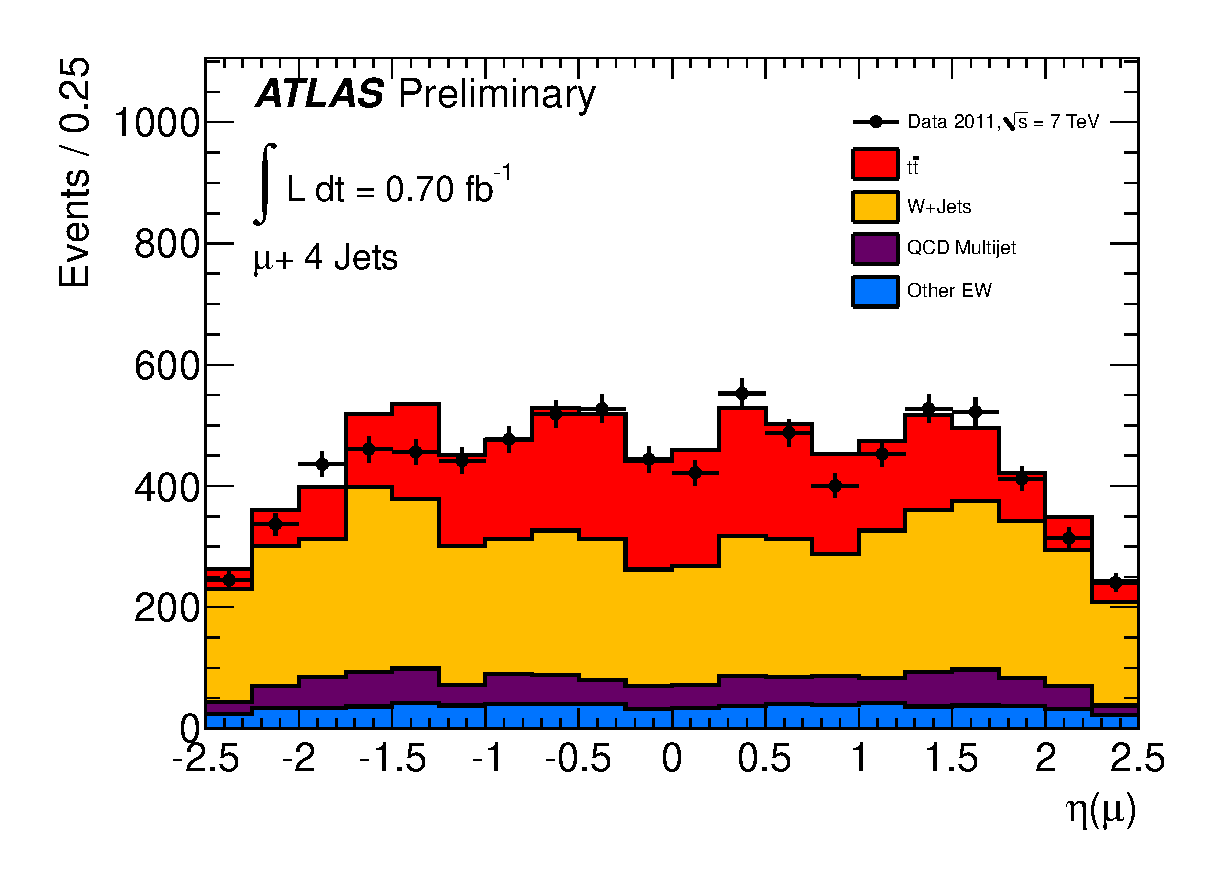
\includegraphics[width=.45\linewidth]{figures/xsection/DiscrimEtaMu4Jets}
    } 
    \subfigure[Aplanarity] {
      % 
      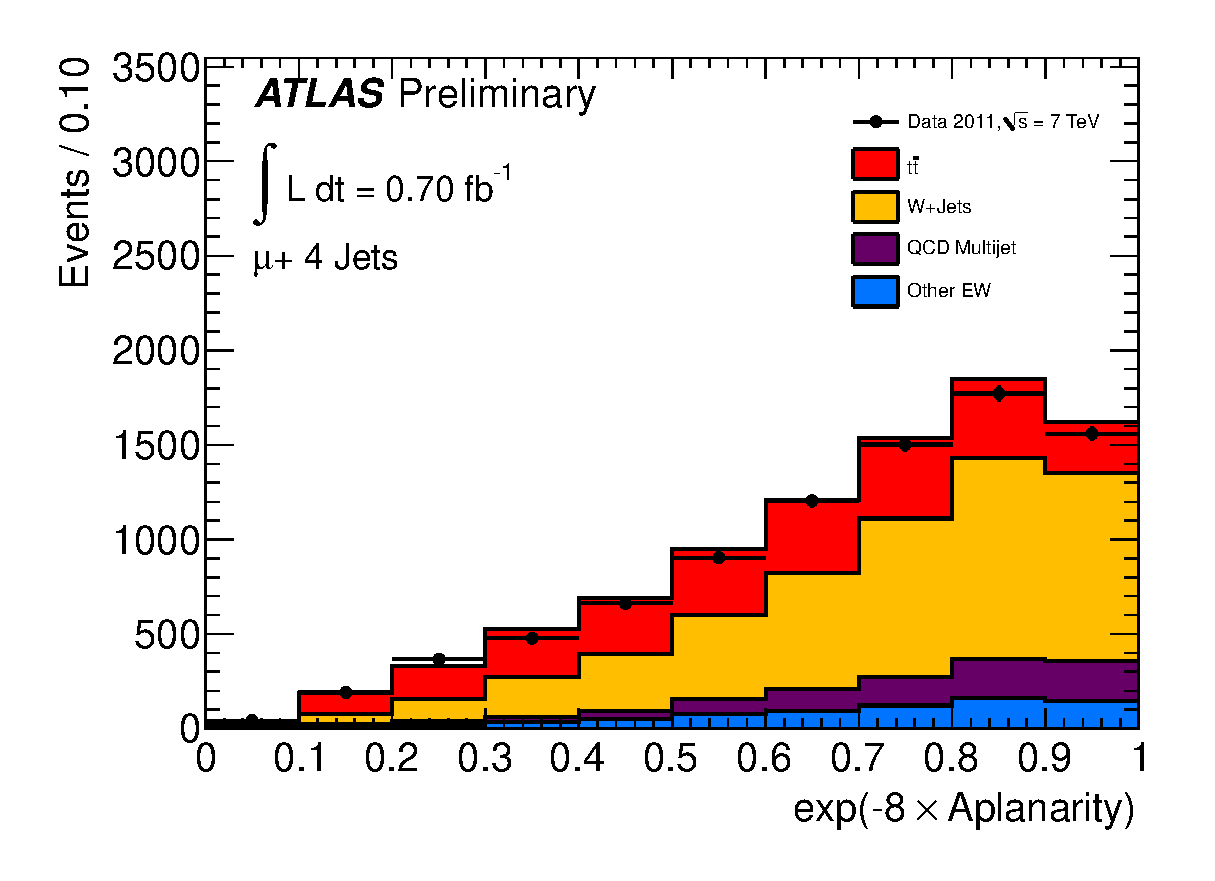
\includegraphics[width=.45\linewidth]{figures/xsection/DiscrimAplanarity4Jets}
    }
    \subfigure[$H_{T,3p}$] {
      % 
      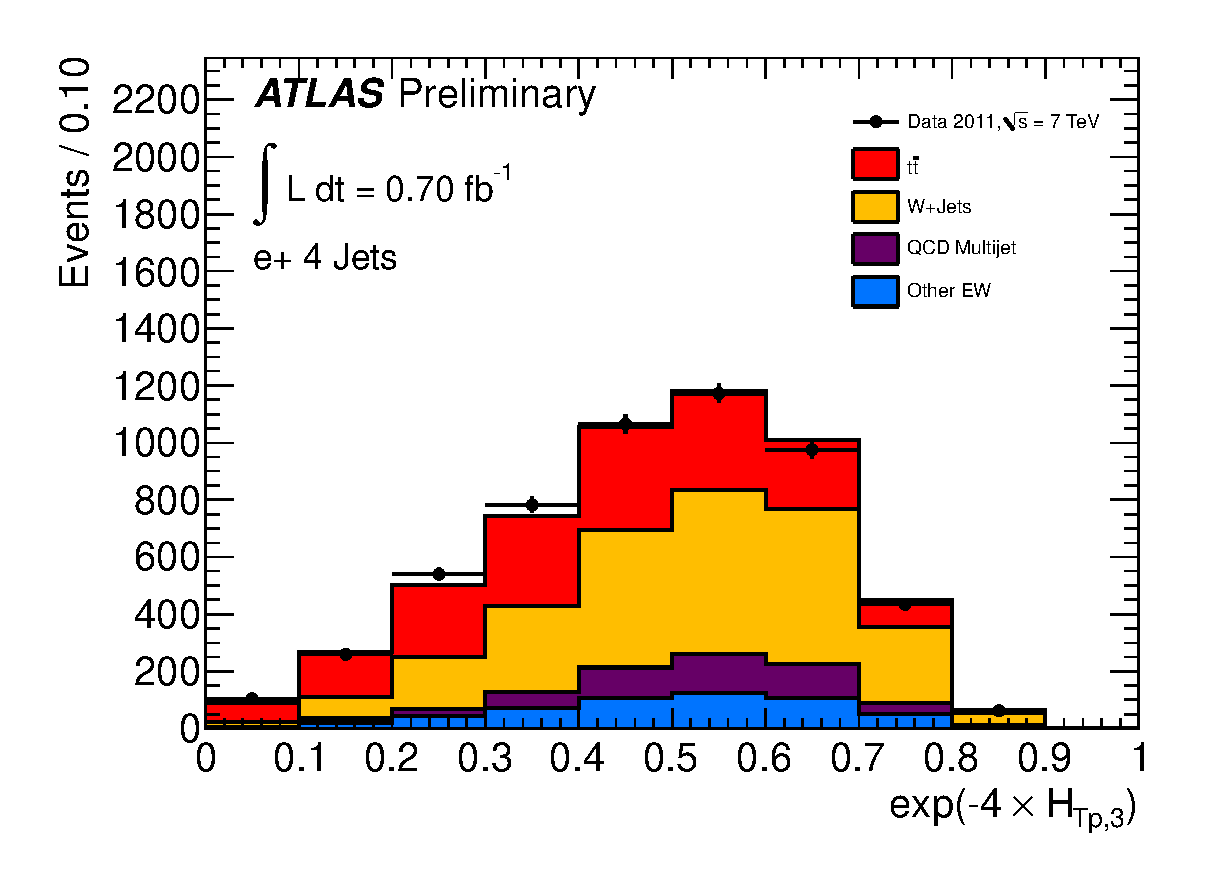
\includegraphics[width=.45\linewidth]{figures/xsection/DiscrimHT34Jets}
    } 
  \end{center}
  \caption{The discriminating variables used in the multivariate likelihood.}
  \label{img:DiscriminatingVariables}
\end{figure}


\begin{figure}
  \begin{center}

    \subfigure[] {
      \includegraphics[width=.95\linewidth]{figures/xsection/LJetsDiscriminantLikelihood}
    }
    \subfigure[] {
      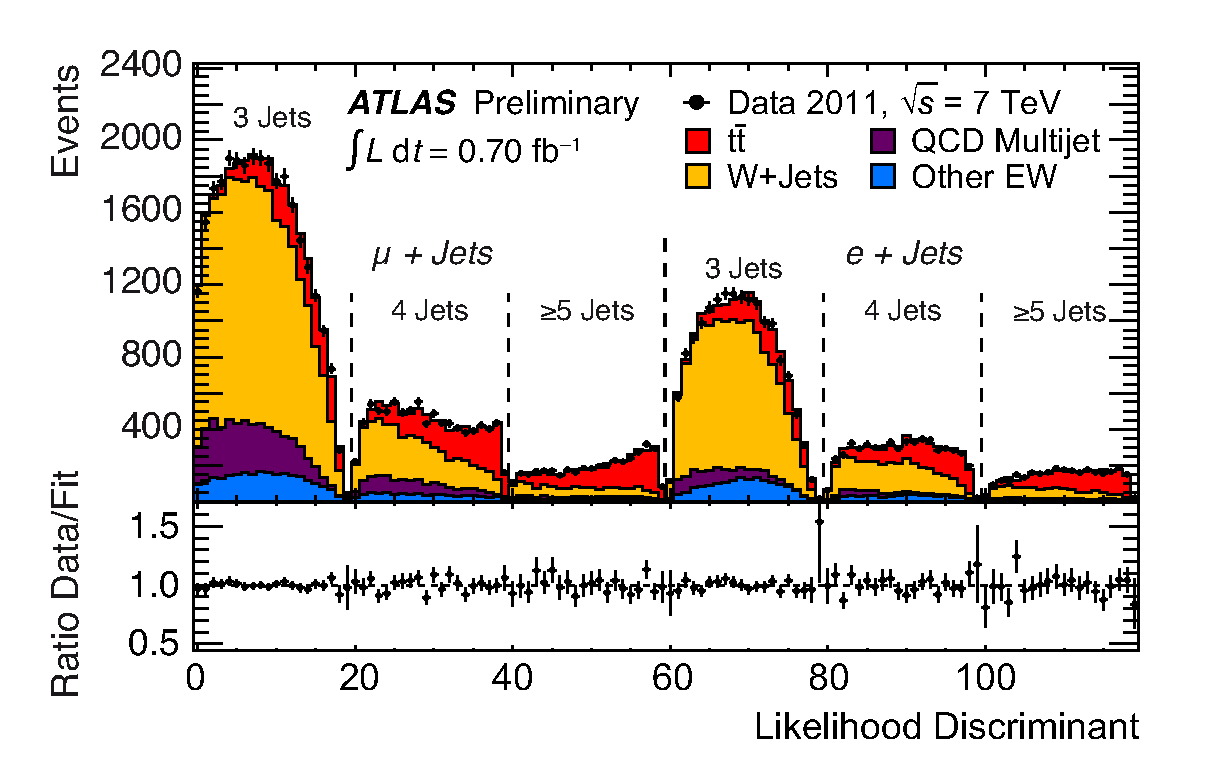
\includegraphics[width=.95\linewidth]{figures/xsection/LJetsFittedLikelihoodDiscriminant}
    }
  \end{center}
  \caption{The multivariate discriminant for $\ttbar$ signal and the dominant $W+Jets$ background.  Distributions are normalized to emphacize the difference in shape between signal and background.}
  \label{img:LJetsLikelihoodDiscriminant}
\end{figure}


\subsection{Systematic Uncertainties}

% The careful and consistent of the effect of systematic uncertainties and their proper paramaterization in a likelihood are crucial to making precise measurements.
The expected distribution of the discriminating variable in each channel and both signal and each background are sensitive to differences in theortical predictions and modeling of experimental effects.
Differences in the expected distributions will lead to differences in the measured cross-section.
Therefore, to incorporate theoretical and experimental uncertainties that will effect the measured cross-section, the expected distributions of the discriminating variable (including their normalizations as a function of integrated luminosity) are paramaterized by a number of terms that each represent on source of systematic uncertainty.
The likelihood function includes the effect of these parameters on the expected distributions as well as terms constraining these parameters, where the level of constraint comes from additional measurements that are made to gauge the size of these systematic uncertainties.
In the lepton+jets analysis, these constraints are modeled as gaussian terms with a mean of 0.0 and a variance of 1.0 (or rather, each paramater is scaled such that its constraint terms can be modeled in this way).

In the lepton+jets analysis, these uncertainties fall into several categories.  
Uncertainties on the cross-sections of backgrounds estimated using monte-carlo lead directly to uncertainties on the number of expected events in each bin of the discriminating variable for a fixed integrated luminosity.
These uncertainties on the cross-sections of the diboson, single-top and Z$+$Jet processes are determined by theoretical studies using Monte-Carlo simulation.
Uncertainties on the normalizations of the data-driven W$+$Jets and QCD backgrounds come from the propogation of statistical uncertainties through the data-driven techniques.
These data-driven normalization uncertainties are considered to be uncorrelated across in the 3 Jets, 4 Jets, and 5+ Jets channels (meaning, the effect is modeled by a separate parameter for each channel, and these parameters each have separate constraint terms and are allowed to move independently in a fit).

Uncertainties on the identification, reconstruction, and measurement of physical objects (jets, leptons, and $\MET$) effect the number of events that are selected, which channels those events may fall into, and the shape of discriminating variables within that channel.
These uncertainties include the energies of reconstructed objects as well as the rate at which they are triggered and identified.
Uncertainties on the measured energies of particles include uncertainties on both the energy scale and the energy resolution (roughly, these correspond to the mean and width of the distribution of measured energy, respectively).
The size of the uncertainties on object energy scale and energy resolution are paramaterized by many parameters of the object, but most importantly its position in the detector (in $\eta$ and $\phi$) and its nominal measured energy. [**]
The effect of energy uncertainties are estimated by rescaling or randomly smearing the energy of objects in Monte-Carlo and obtaining new histograms of the discriminating variables for each background and sample.
Two such sets of template histograms are created for each source of systematic uncertainty corresponding to the effect of a +1 sigma and -1 sigma shift in these parameters (in addition to the nominal histograms, which in this language correspond to a 0 sigma shift in all systematic uncertainties).
The shapes of discriminating histograms for arbitrary shifts in uncertainty parameters are obtained by interpolating between these templates.
Furthermore, uncertainties in the Jet Energy Scale are broken down into subcomponents which consider separately uncertainties on the JES due to the calorimeter, uncertainties due to extrapolating from a low b-jet region to a high b-jet region, the dependence of calibration on pseudorapidity, the modeling of jets across generators, the effect of pile-up, and the effect of the underlying event.

Similarly, uncertainties on the rate at which leptons are identified and triggered are paramaterized by the object's location and energy.[**]
The effect of these uncertainties on the expected distribution of signal and background events estimated from Monte-Carlo are estimatied by scaling the weight of individual events by a factor corresponding to the estimated difference between trigger, reconstruction, and identification rates between Monte-Carlo and data.
These scale factors are derived by studying known processes in data and comparing these processes to Monte Carlo (for leptons, these measurements are performed using Z boson events, where one can create a set of events with a high rate of real to fake leptons).

In addition, uncertainties on the modeling of initial and final state radiation (isr and fsr) in Monte-Carlo, the development of parton showers, and a term generally describing the difference between Monte-Carlo generators.
Finally, uncertainties due to finite Monte-Carlo statistics used to estimate the shapes of backgrounds are considered.

%  W+jets and QCD normalizations are fitted (unconstrained)
%


\subsubsection{Likelihood}

The expected value of the discriminating variable is estimated for every background sample, for every channel, and across all bins.
Using this information, a likelihood function for the measured data in the signal and control regions is created:

\begin{equation}
% L(⃗β, ⃗δ) = 􏰁 P(μk , nk ) × 􏰁 G(β j , ∆ j ) × 􏰁 G(δi , 1)
  L(\vec{\beta}, \vec{\delta}) = \prod Pois(n_{k},\mu_{k}(\vec{\beta},\vec{\delta})) \prod Gauss(\delta_j, \beta_j) \prod( 1, \delta_i),
\end{equation}

where $n_k$ are the values measured in data of each bin of the observable, $\mu_k$ is the expected value of each bin based on a combination of Monte Carlo and data-driven techniques, including the effects of systematic uncertainties.
The systematic uncertainties are paramaterized by two sets of parameters: $\vec{\beta}$, which represent the overall normalizations of backgrounds, and $\vec{\delta}$, which describe various experimental or theoretical uncertainties.

The measured value of the $\ttbar$ cross-section is taken to be the maximum likelihood estimator obtained by fitting the full likelihood, including all channels and systematic parameters, to the observed data distributions.
The uncertianty of this measurement is estimated by finding the interval bounded by the points where the negative log of the profile likelihood ratio crosses $\frac{1}{2}$.

In the context of the lepton$+$jets analysis, a number of the above uncertainties are not considered to be continuous, and therefore one cannot assign a single parameter to describe their effect.
These uncertainties come from differences in the monte-carlo generator used, the hadronization settings, the shapes of the QCD and EW backgrounds, and the effect of finite monte-carlo statistics.
Therefore, these uncertainties are not paramaterized in the lepton+jets likelihood.
Instead, they are evaluated outside of the likelihood fit by generating toy data and evaluating the difference in the uncertainty on the top quark cross-section due to their inclusion.
These uncertainties are later added in quadrature to the uncertainty obtained from the likelihood fit to obtain the total uncertainty on the measured cross-section.


\subsubsection{Results}

This likelihood function, which simultaneously describes all bins across channels for the discriminating variables, is fit to the observed data.
The fitted value of the $\ttbar$ cross section and its uncertainties due to statistical, systematic, and luminosity effects, is found to be $\sigma_{\ttbar} = 179.0 ^{+7.0}_{-6.9}(stat+sys) \pm 6.6 (lumi)$ pb.

Additional uncertainties that are not paramaterized in the Likelihood were added in quadrature to the fitted uncertainties.
These additional uncertainties consist of Generator Hadronization, QCD shape, W shape, and Monte Carlo statistics.

Including these effects, the total uncertainty on the measurement is given by:

$\sigma_{\ttbar} = 179.0 \pm 9.8 (stat + syst) \pm 6.6 (lumi) pb = 179.0 \pm 11.8$ pb.

%%  σtt ̄ =
%% 179.0+7.0 (stat + syst) ± 6.6 (lumi) pb .

%% The combined fit of the six analysis channels to the likelihood discriminant distribution in data in-
%% cluding all systematic uncertainties treated within the fit yields a tt ̄ production cross section of σtt ̄ =
%% 179.0+7.0 (stat + syst) ± 6.6 (lumi) pb . The result of the fit is shown in Fig. 7 and demonstrates an excel- −6.9
%% lent agreement between data and the background and tt ̄ signal model. After including uncertainties that are not part of the fit, σtt ̄ is measured to be
%% σtt ̄ = 179.0±3.9 (stat)±9.0 (syst)±6.6 (lumi) pb = 179.0±9.8 (stat + syst)±6.6 (lumi) pb = 179.0±11.8 pb.


\subsection{Dilepton}


\subsection{Combination}



\subsubsection{Lepton + Jets Likelihood}


\label{sec:lepjets}

%The likelihood function for the single-lepton channel is formed  the $e$+jets and $\mu$+jets models, taking into account common systematic uncertainties.  
The single-lepton channel, which consists of $e$+jets and $\mu$+jets final states, is described by a single likelihood function.
This likelihood function consists of the parameter of interest, $\sigma_{\ttbar}$, and 45 nuisance parameters $\vec{\alpha}$, 
which are together denoted $\vec{\theta} = (\sigma_{\ttbar}, \vec{\alpha})$.
The maximum likelihood estimator of this single-lepton combination is denoted $\hat{\vec{\theta}}$.
The largest sources of systematic uncertainty in the single-lepton channel come from the Monte Carlo generator for signal, the jet energy scale, and the modeling of initial-state and final-state radiation.
Uncertainties that affect the background only, including uncertainties on the shape of $W+$jets and QCD templates, contribute less than those affecting signal only.
More information on the cross-section measurement using single-lepton final states can be found in reference~\cite{lepjetsCONF}.

For the purposes of the six-measurement combination, the likelihood from the single-lepton channels is approximated using a multivariate Gaussian.
This approximation facilitates the combination with the dilepton and all-hadronic likelihoods, which are implemented in a different software framework.  
Figure~\ref{fig:ljets_combined} shows $-\log\lambda(\sigma_{\ttbar})$ vs. $\sigma_{\ttbar}/\sigma_{\rm SM}$ for the single-lepton model using both the exact and the approximate likelihood.
It can be seen that the likelihood is very symmetric and parabolic, indicating that a multivariate Gaussian is a good approximation to the likelihood function. 
The covariance matrix used to construct the multivariate Gaussian comes from the Hessian matrix of the negative log-likelihood function evaluated at the best fit point:

% The largest contribution to the systematic uncertainty on the begin  comes from the choice of the signal MC generator followed by the uncertainties on the jet energy scale calibration and the modeling of initial and final state radiation.

% The uncertainties on the background modeling come from the uncertainty on the shape of W+jets and QCD templates


%  \begin{equation}
%  V_{ij}^{-1} = - \frac{\partial^2 }{\partial \theta_i \partial \theta_j} \log L(\vec{\theta})\; \bigg | \; {\hat{\vec{\theta}}} \; .
%  \end{equation}
%\end{minipage}
%\hspace{0.5cm}
%\begin{minipage}{0.7\linewidth}
%  \begin{equation}
%  L_{l+\rm jets}(\vec{\theta}) = G(\hat{\vec{\theta}}\, |\, \vec{\theta}, V) = \frac{1}{(2\pi)^{k/2} | V|^{1/2}} \exp\left( -\frac{1}{2} (\hat{\vec{\theta}} - \vec{\theta})^T  V^{-1} (\hat{\vec{\theta}} - \vec{\theta})  \right) \;, 
%  \end{equation}
%  \end{minipage}


\begin{equation}
  V_{ij}^{-1} = - \frac{\partial^2 }{\partial \theta_i \partial \theta_j} \log L(\vec{\theta})\; {\bigg | \;}_{\hat{\vec{\theta}}} \; \quad .
\end{equation}
With the covariance matrix, one can construct the multivariate Gaussian likelihood 
\begin{equation} \label{eqn:ljetsLikelihood}
  L_{l+\rm jets}(\vec{\theta}) = G(\hat{\vec{\theta}}\, |\, \vec{\theta}, V) = \frac{1}{(2\pi)^{k/2} | V|^{1/2}} \exp\left( -\frac{1}{2} (\hat{\vec{\theta}} - \vec{\theta})^T  V^{-1} (\hat{\vec{\theta}} - \vec{\theta})  \right) \;, 
\end{equation}
where $k=46$ is the dimensionality of the parameter space.  
Uncertainties that are evaluated outside of the fit in in reference~\cite{lepjetsCONF} are here modeled as factors which scale $\sigma_{\ttbar}/\sigma_{\rm SM}$ and are described by Gaussian terms.
%Uncertainties that are evaluated outside of the fit in the single-lepton analysis are here modeled as scalings on $\sigma_{\ttbar}/\sigma_{\rm SM}$ and are constrained by Gaussian terms.
%Uncertainties that are evaluated outside of the fit in the single-lepton analysis are here modeled as parameterized uncertainties on $\sigma_{\ttbar}/\sigma_{\rm SM}$ in the multivariate gaussian likelihood.


\begin{figure}[htbp]
  \begin{center}
    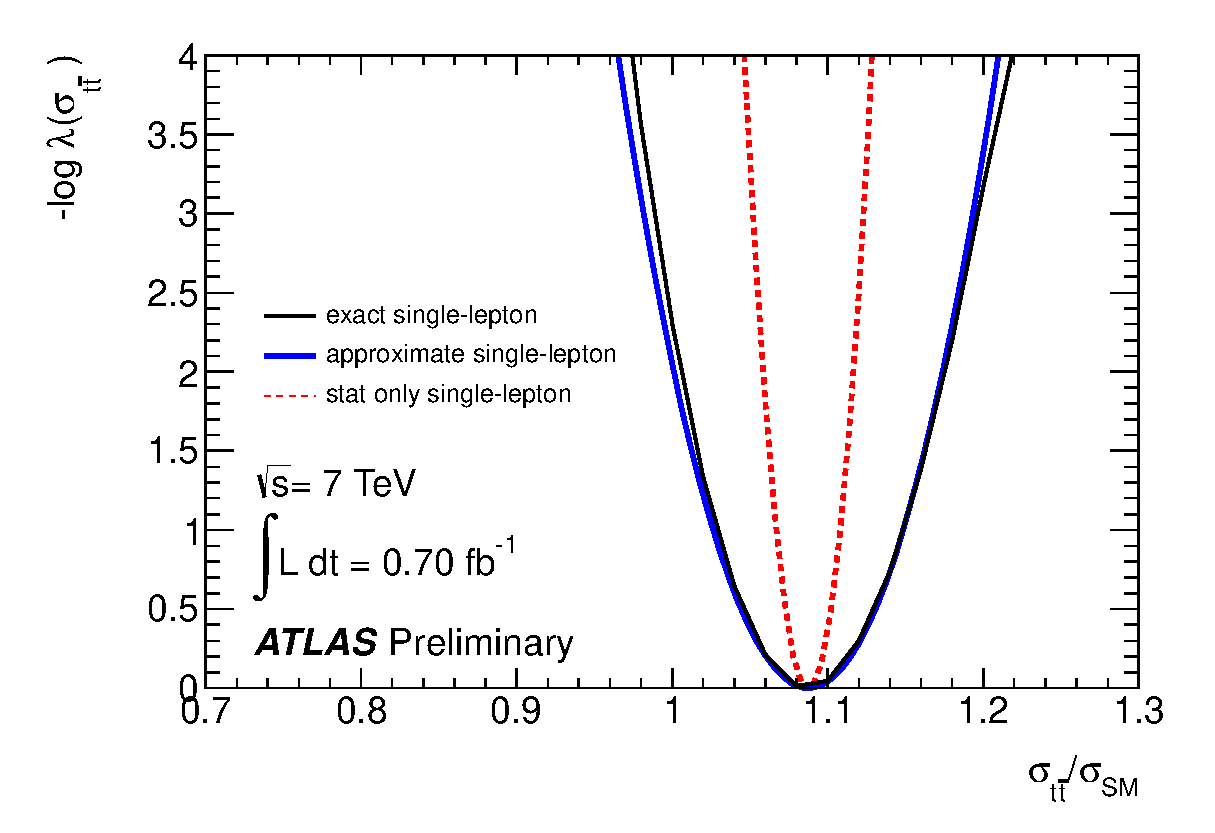
\includegraphics[width=.5\textwidth]{figures/comb/ljets_likelihood_curve}
    \caption{Graph of $-\log\lambda(\sigma_{\ttbar})$ vs. $\sigma_{\ttbar}/\sigma_{\rm SM}$ for both the exact (black, solid) and approximate (blue, solid) $l$+jets likelihood~\cite{lepjetsCONF}.  The same graph using the approximate likelihood without systematic uncertainties (red, dashed) is also shown.  The likelihoods shown here do not include systematics that are evaluated outside of the fit.}
    %\includegraphics[width=.5\textwidth]{figures/comb/ljets_likelihood_curve_ljets_onePlot.eps}
    %\caption{Graph of $-\log\lambda(\sigma_{\ttbar})$ vs. $\sigma_{\ttbar}/\sigma_{\rm SM}$ for the $l$+jets combined likelihood.}
    \label{fig:ljets_combined}
  \end{center}
\end{figure}

%\begin{figure}[htbp]
%  \begin{center}
%    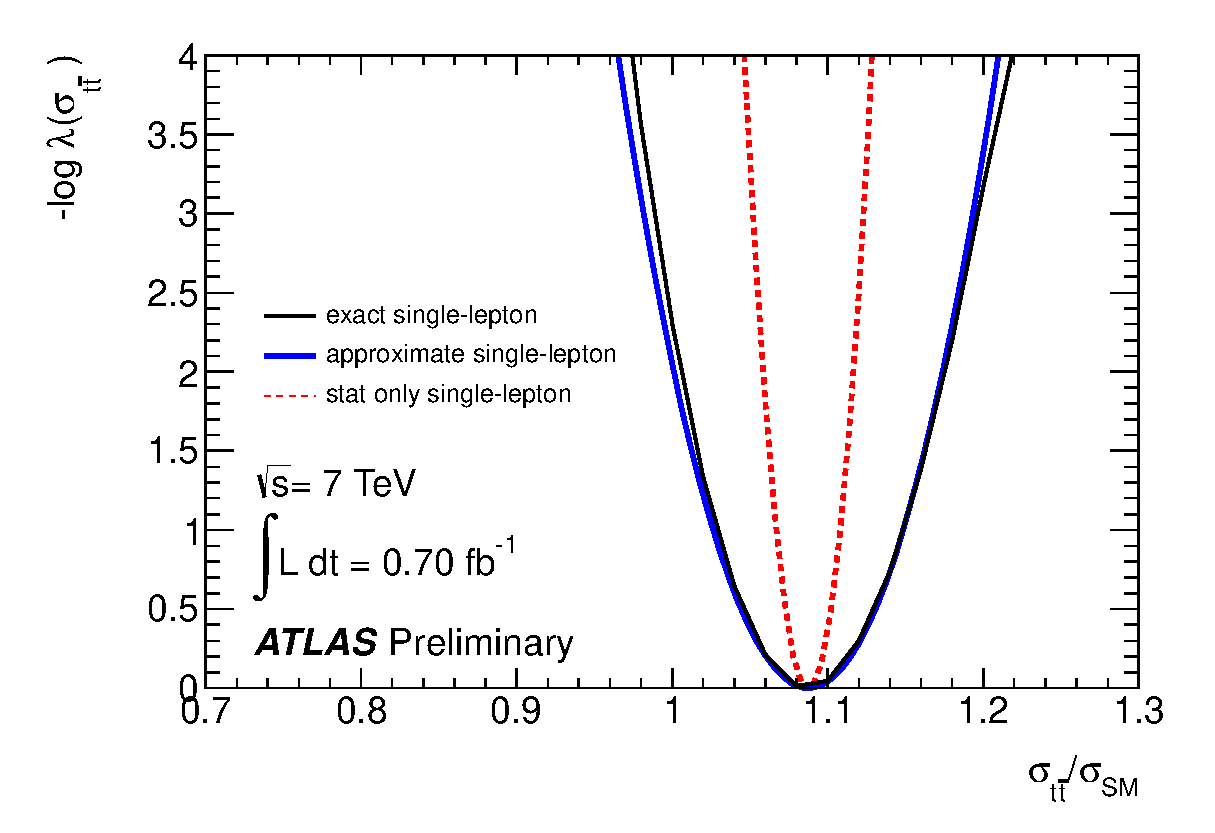
\includegraphics[width=.5\textwidth]{figures/comb/ljets_likelihood_curve.eps}
%    \caption{Graphs of $-\log\lambda(\sigma_{\ttbar})$ vs. $\sigma_{\ttbar}/\sigma_{\rm SM}$ from the $e$+jets (green, dashed), $\mu$+jets (blue, dashed), and $l$+jets combined likelihood (black, solid).  The likelihoods do not include systematics that are evaluated outside of the fit.}
%    %\includegraphics[width=.5\textwidth]{figures/comb/ljets_likelihood_curve_ljets_onePlot.eps}
%    %\caption{Graph of $-\log\lambda(\sigma_{\ttbar})$ vs. $\sigma_{\ttbar}/\sigma_{\rm SM}$ for the $l$+jets combined likelihood.}
%    \label{fig:ljets_combined}
%  \end{center}
%\end{figure}



% INT ONLY
Internal consistency checks were preformed to ensure the validity of this approximation.  Figure~\ref{fig:ljets_profile} demonstrates that the parameters of the approximate single-lepton likelihood are consistent with the exact likelihoods of the $e$+jets and $\mu$+jets channels, which are shown to be well approximated by a Gaussian.
Each graph contains a verticle line representing the fitted value of $\sigma/\sigma_{\rm SM}$.
The graphs of $\hat{\hat{\alpha}}_j$ vs. $\sigma/\sigma_{\rm SM}$  using the exact likelihoods of the $e+\textrm{jets}$, $mu+\textrm{jets}$, and combined single-lepton channel are shown.
The red curve represents the graph of $\hat{\hat{\alpha}}_j$ vs. $\sigma/\sigma_{\rm SM}$ using the approximated single-lepton likelihood.
One can see that the curves generated using the exact single-lepton likelihood (black) closely follow the curves generated using the approximate single-lepton likelihood (red).
In particular, the values and slopes of those curves match each other well near the fitted value of $\sigma/\sigma_{\rm SM}$, about which the multivariate approximation is evaluated. 

% INT ONLY
\begin{figure}[htbp]
  \begin{center}
    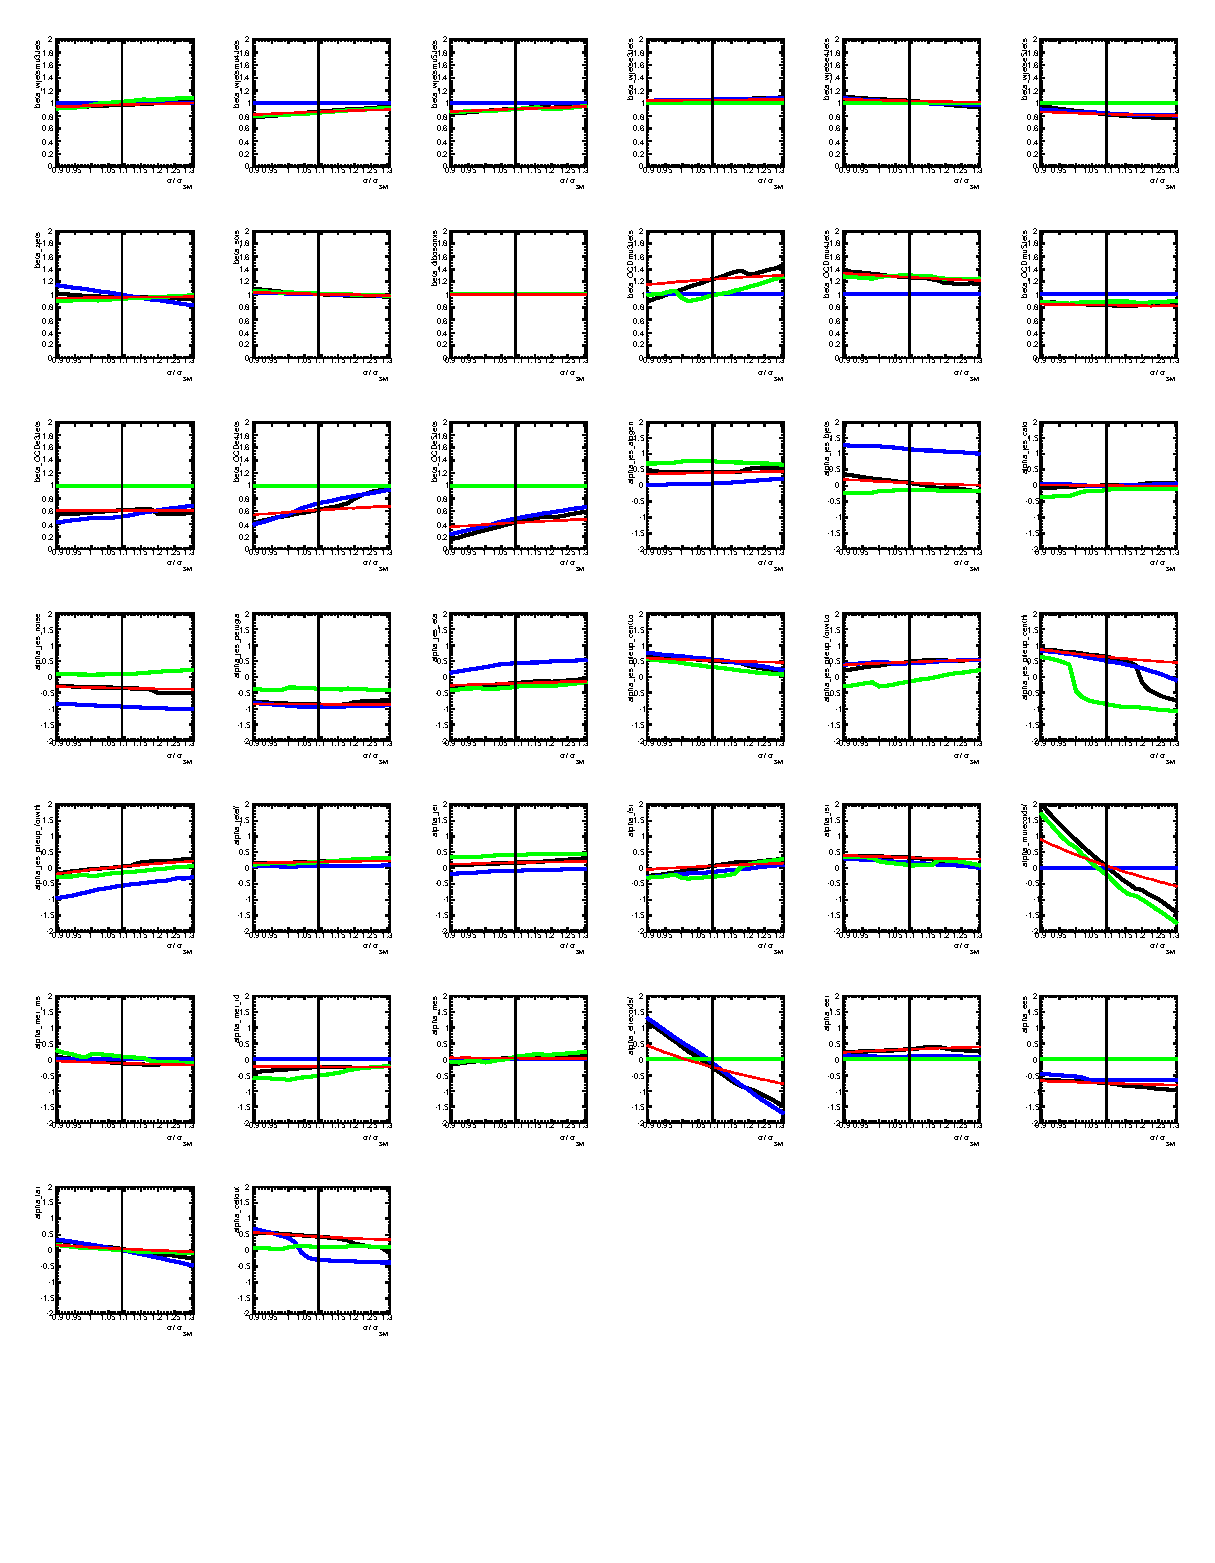
\includegraphics[width=\textwidth]{figures/comb/LJetsProfilePlots}
    \caption{The conditional maximum likelihood estimates $\hat{\hat{\alpha}}_j$ vs. $\sigma/\sigma_{\rm SM}$ for the single lepton analyses.  The results from the full likelihood of the individual channels $e+\textrm{jets}, \mu+\textrm{jets}$ are shown in blue and green, respectively, and the combined result is shown in black.  The red curve shows the approximation of the combined likelihood function with a multivariate Gaussian.  The vertical black line indicates the best fit signal cross-section, where the Gaussian approximation and the full combined likelihood should (and do) meet.  The scale of the $\alpha$ parameters is such that $\pm 1$ indicates $\pm 1\sigma$ uncertainty in the source of the systematic.}
    \label{fig:ljets_profile}
  \end{center}
\end{figure}

\subsubsection{Dilepton}
\label{sec:dilep}


The likelihood function for each of the dilepton channels consists of a single Poisson term for the number of observed events with $\ge2$ jets and several Gaussian constraint terms for the nuisance parameters $\vec{\alpha}$.   
These nuisance parameters are defined such that the nominal value of a systematic uncertainty corresponds to $\alpha_j = 0$ and a one standard deviation shift corresponds to $\alpha_j = \pm 1$.
These parameters are therefore constrained by Gaussian terms with means of 0 and standard deviations of 1.
Similarly, the parameter corresponding to the integrated luminosity, $\lum$, is constrained by a Gaussian term whose mean is the nominal value of the integrated luminosity, $\lum_{0}$, and whose standard deviation, $\sigma_{\lum}$, is equal to the uncertainty on the integrated luminosity.
The combined likelihood is given by the product of the Poisson terms and the Gaussian constraint terms

\begin{equation}\label{Eq:dileplikelihood}
  L_{ll}(\sigma_{\ttbar}, \lum, \vec{\alpha}) = \text{Gaus}(\lum_0 | \lum, \sigma_\lum)\, \prod_{i\in \{ ee,\mu\mu,e\mu\} }  \text{Pois}(N^{\text{obs}}_i \,|\, N^{\text{exp}}_{i, \text{tot}}(\vec{\alpha})\,) \,  \prod_{j\in \text{syst}} \text{Gaus}( 0 \,|\, \alpha_{j}, 1) \,,
\end{equation}
%where Pois is the Poisson distribution, Gaus is the Gaussian distribution, and the constraint terms on common systematic uncertainties are only included once.  
where constraint terms on common systematic uncertainties are only included once.  
%The Gaussian terms that constraint the parameters describing the effect of systematic uncertainties, $alpha_j$, are defined such that the measured value of a systematic corresponds to $alpha_j = 0$  their measured value in data i
The variation in the expected number of events from the signal and each background process is estimated from dedicated studies of each of the systematic effects.  
The total number of expected events, $N^{\text{exp}}_{i,\text{tot}}(\alpha_j)$, is then parametrized via piece-wise linear interpolation in the nuisance parameters $\alpha_j$ associated with each source of systematic uncertainty using the RooFit/RooStats software package~\cite{Verkerke:2003ir,Moneta:2010pm}.

%\begin{equation}\label{Eq:alphaInterpolation}
%N^{\text{exp}}_{i, \text{tot}}(\vec{\alpha}) = \sum_{\text{background}} N^{\text{exp}}_{i} (1 + \sum_{j} \alpha_{j} ( \mathbbm{1}_{ \alpha_{j} > 0} \, \Delta N^{+}_{j} - \mathbbm{1}_{ \alpha_{j} < 0} \, \Delta N^{-}_{j}   ) ) \, ,
%\end{equation}
%where $\mathbbm{1}$ is the indicator function whose value is 1 or 0 if its argument is true or false, respectively, and $\Delta N^{+}_{j}$ and $\Delta N^{-}_{j}$ are the differences in the expected number of events due to an updward or downward fluctuation of one standard deviation of the $j^{th}$ nuisance parameter. 

\begin{eqnarray}\label{Eq:alphaInterpolation}
N^{\text{exp}}_{i, \text{tot}}(\vec{\alpha}) &=& \sum_{\text{background}} N^{\text{exp}}_{i} (1 + \sum_{j} \alpha_{j} \, \Delta N_j  ) \, \\ 
\Delta N_j &=& \begin{cases} \Delta N^{+}_{j}, & \mbox{if } \alpha_{j} > 0  \\ \Delta N^{-}_{j}, & \mbox{if } \alpha_{j} < 0 \end{cases} , 
\end{eqnarray} 
where $\Delta N^{+}_{j}$ and $\Delta N^{-}_{j}$ are the differences in the expected number of events due to an upward or downward fluctuation of one standard deviation of the $j^{th}$ nuisance parameter. 

The dilepton likelihood function contains 65 parameters, including the parameter of interest, $\sigma_{\ttbar}$, the integrated luminosity, $\lum$, and 63 other nuisance parameters.
The profile likelihood ratios for the individual channels as well as the dilepton combination are shown in Figure~\ref{fig:dilep_profiles}.  
The dominant systematic uncertainties for the dilepton analysis are lepton identification efficiencies, fake lepton rates, modeling of the signal, and jet energy scale, which is modeled identically in the single-lepton and dilepton channels.
%To match the single-lepton analysis, the effect of the jet energy scale uncertainty is parameterized by several components, each of which is considered independent.
More information on the measurement using dilepton final states can be found in reference \cite{dileptCONF}.

\begin{figure}[htbp]
  \begin{center}
    \subfigure[$ee$]{       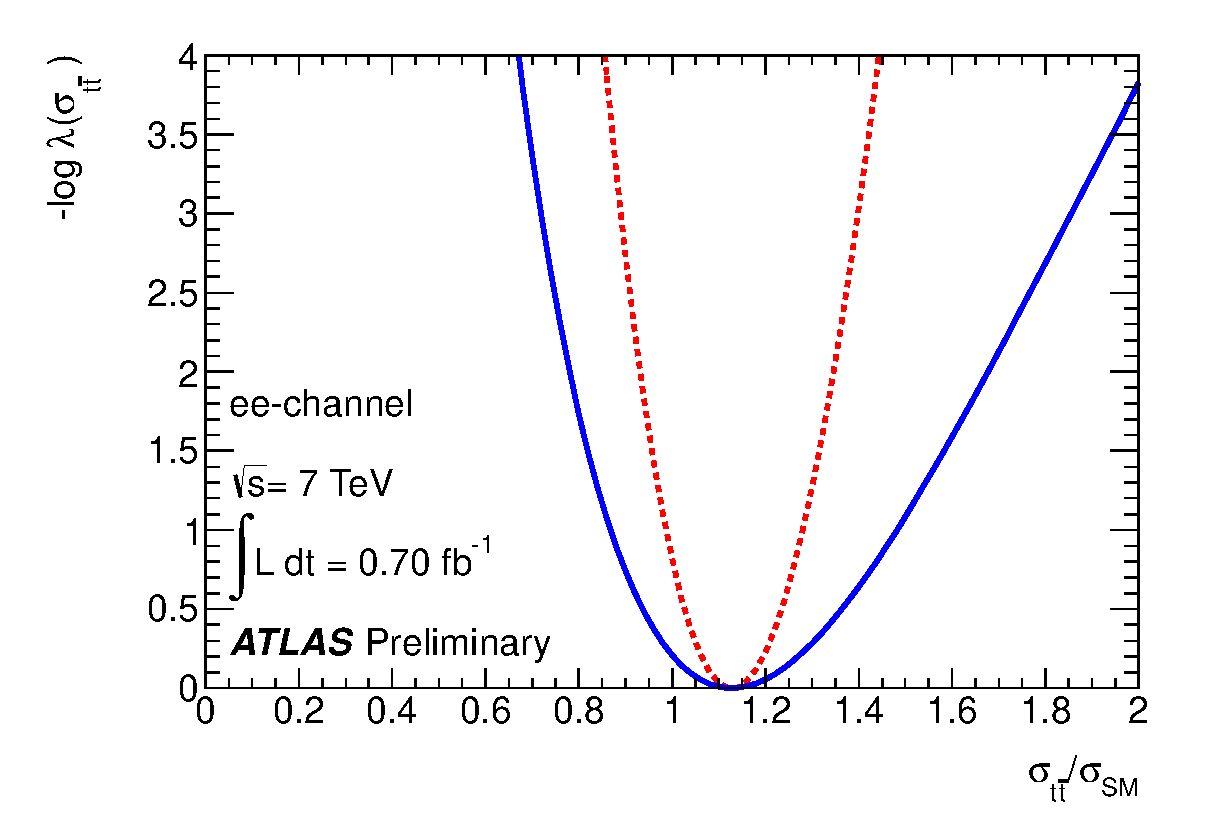
\includegraphics[width=.40\textwidth]{figures/comb/top_dilepton_ee_forComb_profileLR} }
     \subfigure[$\mu \mu$]{ \includegraphics[width=.40\textwidth]{figures/comb/top_dilepton_mm_forComb_profileLR} }\\
     \subfigure[$e \mu$]{   \includegraphics[width=.40\textwidth]{figures/comb/top_dilepton_em_forComb_profileLR} }
     \subfigure[Combined]{  \includegraphics[width=.40\textwidth]{figures/comb/top_dilepton_combined_forComb_profileLR} }\\
    \caption{Graphs of $-\log\lambda(\sigma_{\ttbar})$ vs. $\sigma_{\ttbar}/\sigma_{\rm SM}$ with (blue, solid) and without (red, dashed) systematic uncertainties for the individual channels $ee$ (a), $\mu\mu$ (b), and $e\mu$ (c), and the three-channel combined fit (d).}
    \label{fig:dilep_profiles}
  \end{center}
\end{figure}





% INT ONLY
 \begin{figure}[htbp]
   \begin{center}
     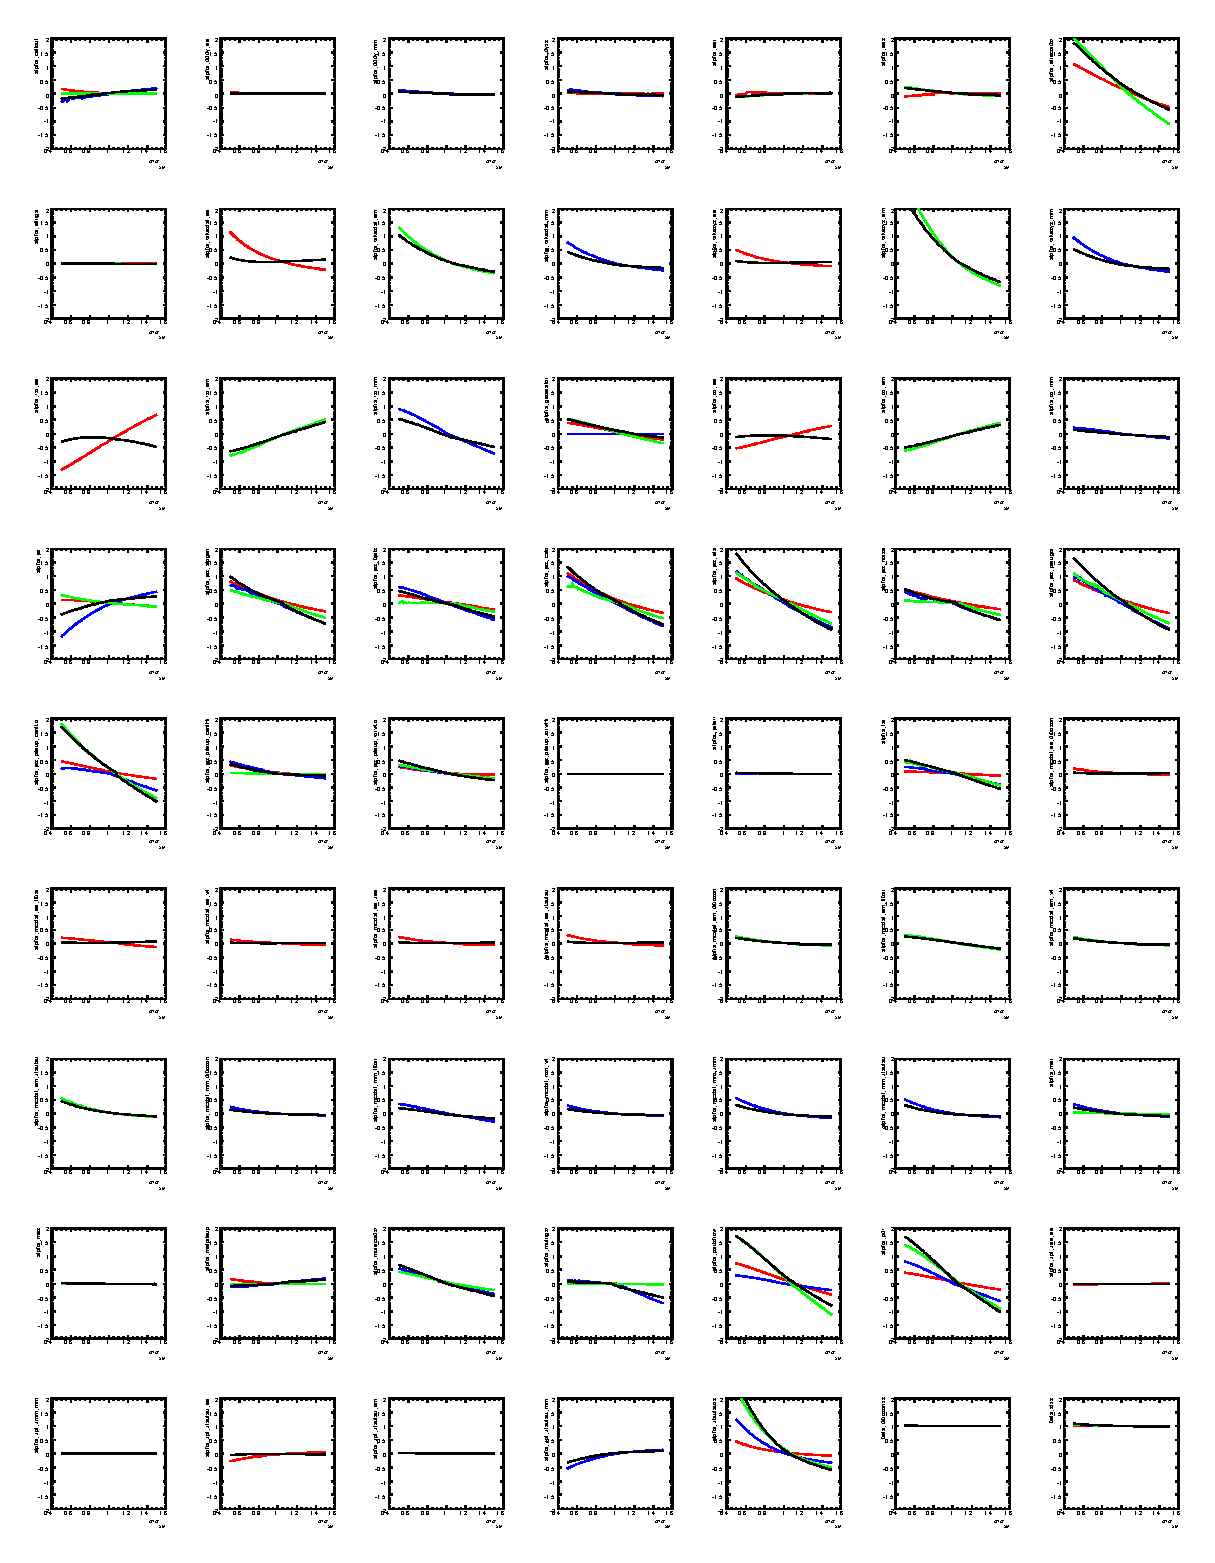
\includegraphics[width=\textwidth]{figures/comb/DilepProfilePlots}
    \caption{The conditional maximum likelihood estimates $\hat{\hat{\alpha}}_j$ vs. $\sigma/\sigma_{\rm SM}$ for the dilepton analyses.  The individual channels $ee, \mu\mu, e\mu$ are shown in red, blue, and green, respectively, and the combined result is shown in black.  The scale of the $\alpha$ parameters is such that $\pm 1$ indicates $\pm 1\sigma$ uncertainty in the source of the systematic.}
     \label{fig:dilepton_profile}
   \end{center}
 \end{figure}


\subsubsection{all hadronic}
\label{sec:allhad}

The top quark cross-section is measured in the all-hadronic channel by performing a binned likelihood fit of signal and background templates to data.
The observable described by these templates is based on the reconstructed top-quark mass per event:
% of a $\chi^2$ of the reconstructed top-quark mass per event as a   discriminant''
% the minimum $\chi^2$d of the reconstructed top-quark mass:
%  kinematic fit assuming the $\ttbar$ event hypothesis
% $\chi^2$ distribution of the reconstructed top-quark mass to data

\begin{equation}\label{Eq:chisquare}
  \chi^2 =  \frac{ \left(m_{j_1, j_2} - m_{W}\right)^2}{\sigma_W^2} + \frac{ \left(m_{j_1, j_2, b_1} - m_{t}\right)^2}{\sigma_t^2} + \frac{ \left(m_{j_3, j_4} - m_{W}\right)^2}{\sigma_W^2} + \frac{ \left(m_{j_3, j_4, b_2} - m_{t}\right)^2}{\sigma_t^2},
  \end{equation}
where the particular jet combination used per event is the one that minimizes this sum~\cite{allhadCONF}.
% where the choice of jet labeling per event is the one that minimizes this $\chi^2$d.
% where the set of jets labeling that minimizes this $\chi^2$d per event is chosen.
% where the choice of jets per event is that which minimize this $\chi^2$d.
% where the combination of reconstructed objects that minimize this $\chi^2$ are used per event~\cite{allhad}.

The likelihood function for the all-hadronic channel consists of a product of Poisson terms, 
one for each of the 15 bins in the distribution of the $\chi^2$ value defined by equation~\ref{Eq:chisquare} above. 
The mean value for each bin is the sum of the signal and background templates, including the parametrized effects of systematic uncertainties.
%one for each of the 15 bins, describing the height of the $\chi^2$ distribution.
%The mean height for each bin is the sum of the signal and background templates, including the parametrized effects of systematic uncertainties.
%The signal template is generated using Monte Carlo simulation, and the background template, 
The signal template is generated using Monte Carlo simulation and the background template, which models the $\chi^2$ distribution in QCD multijet events, is extracted using a data-driven technique.
%These template distributions are each scaled by the luminosity, which is Gaussian constrained in the likelihood fit.
In total, the all-hadronic likelihood contains 22 parameters, including $\sigma_{\ttbar}$, the integrated luminosity, and 20 other nuisance parameters.
%The likelihood function used in this note was built using the RooFit/RooStats software package [9, 10]

The size of the systematic uncertainties in the all-hadronic channel are measured by fitting alternative templates of signal and background, 
each representing the plus or minus one standard deviation shift of an individual source of systematic uncertainty.
In the likelihood used for the combination, each source of systematic uncertainty enters as an overall scaling of the signal or background normalization,
the size of which is based on the measured uncertainties in the all-hadronic channel.
%These scalings are constrained by Gaussian terms such that a one standard deviation shift in the underlying parameter has an effect on the signal or background normalization equal to the measured size of each systematic.
The likelihood for the all-hadronic channel is given by

%\begin{equation}\label{Eq:dileplikelihood}
%  L_{had}(\sigma_{\ttbar}, \lum, \alpha_{j}) = \text{Pois}(N^{obs} \,|\, s(\alpha_j) + b(\alpha_j)) \prod_{i\in bins} \text{Pois}(n_{i} \,|\, s(\alpha_j) f_{i}^{s} \,+\, b(\alpha_j) f_{i}^{b})  \prod_{j\in \text{syst}} \text{Gaus}( 0 \,|\, \alpha_{j}, 1) \, \text{Gaus}(\lum_0 | \lum, \sigma_\lum)\,
%\end{equation}
\begin{equation}\label{Eq:dileplikelihood}
  L_{\text{had}}(\sigma_{\ttbar}, \lum, \vec{\alpha }) = \text{Gaus}(\lum_0 | \lum, \sigma_\lum)\, \prod_{i\in \text{bins}} \text{Pois}(n_{i} \,|\, s_{i}(\vec{\alpha}) \,+\, b_{i}(\vec{\alpha}))  \prod_{j\in \text{syst}} \text{Gaus}( 0 \,|\, \alpha_{j}, 1) \,  ,
\end{equation}
where $s_{i}(\vec{\alpha})$ and $b_{i}(\vec{\alpha})$ are the expected number of events from signal and background in the $i^{th}$ bin and $n_{i}$ is the observed number of events in the same bin. 

The largest sources of systematic uncertainty in the all-hadronic model are the jet energy scale, the $b-$tagging efficiency, and modeling of initial-state and final-state radiation.
Other significant sources of uncertainty include the jet energy resolution, the efficiency of the multijet trigger, and modeling of the multijet background.
Further details on cross-section measurement using all-hadronic final states can be found in reference~\cite{allhadCONF}.
The likelihood function for the all-hadronic channel is shown in Figure ~\ref{fig:allhad_likelihood}.

\begin{figure}[htbp]
  \begin{center}
    \includegraphics[width=.40\textwidth]{figures/comb/allhadronic_likelihood_curve}
  \caption{Graph of $-\log\lambda(\sigma_{\ttbar})$ vs. $\sigma_{\ttbar}/\sigma_{\rm SM}$ with (blue, solid) and without (red, dashed) systematic uncertainties for the all-hadronic channel.}
  \label{fig:allhad_likelihood}
  \end{center}
\end{figure}



\subsubsection{Combined Likelihood}
\label{sec:comb}

The component analyses share several common sources of systematic uncertainty:
\begin{itemize}
\item electron and muon identification efficiencies,
\item electron energy scale and resolution,
\item muon momentum scale and resolution,
\item Monte Carlo generator, modeling of initial-state and final-state radiation,
\item jet energy resolution, jet energy scale, and jet efficiency,
\item calculation of missing transverse energy,
\item sporadic hardware failures which are not modeled in simulation,
\item background contributions from diboson and single top-quark events,
\item parton distribution functions and parton shower modeling,
\item integrated luminosity.
\end{itemize}

% The constraint terms $G(0|\alpha_j,1)$ associated with these common uncertainties cannot be double-counted.  

Sources of systematic uncertainty which are shared between channels are taken to be fully correlated.
The sources of uncertainty related to the modeling of the $\ttbar$ signal that are listed above are taken to be fully correlated because common Monte Carlo generators, parton distribution functions, and parton shower software were used across the single-lepton, dilepton, and all-hadronic analyses.
Experimental uncertainties, such as energy scales and identification efficiencies, that are listed above are correlated because they represent quantities that act coherently across channels and because they are modeled and evaluated using common techniques.
%  Systematic uncertainties that are correlated across channels
Constraint terms that are common to one or more of the single-lepton, dilepton or all-hadronic likelihoods appear only once in the full six-measurement likelihood.
%must be removed when forming the six-channel combination. 
% Because the likelihood function from the single-lepton analysis is approximated by a single multivariate Gaussian, constraint terms in the dilepton or all-hadronic likelihoods that are shared by the single-lepton likelihood must be removed when forming the six-channel combination. 
% Before combining, the dependence of the conditional maximum likelihood estimates, $\hat{\hat{\alpha}}_j$, as a function of $\sigma_{\ttbar}/\sigma_{\rm SM}$ were compared for the dilepton and single-lepton channels.  
% Those studies did not indicate any unexpected tension in the shared nuisance parameters that would indicate incompatible results.

%The final six-channel likelihood (equation \ref{Eq:combinedlikelihood}) is formed from a product of the approximate single-lepton likelihood, $L_{l+\rm jets}$, which includes the parameter of interest, $\sigma_{\ttbar}$, and 45 nuisance parameters (25 of which are shared with the dilepton channels, including a luminosity constraint), the Poisson terms corresponding to the cut-based analyses for the dileptons (which depend on the parameter of interest), the all-hadronic likelihood and Gaussian constraints for the remaining 28 nuisance parameters that only affect the dilepton channels.  
The final six-measurement likelihood (equation \ref{Eq:combinedlikelihood}) is formed from a product of the approximate single-lepton likelihood, the Poisson terms corresponding to the cut-based dilepton analyses, the template-based all-hadronic likelihood, and Gaussian constraint terms for the 43 nuisance parameters that are not constrained by the single-lepton likelihood.

%In total, there are 74 parameters in the six-channel combined fit.

\begin{eqnarray} \label{Eq:combinedlikelihood} \nonumber
  L_{\text{comb}}(\sigma_{\ttbar}, \lum, \vec{\alpha}) &=& L_{l+\rm jets}(\sigma_{\ttbar},\lum, \vec{\alpha})  \prod_{i\in \{ ee,\mu\mu,e\mu\} } 
   \text{Pois}(N^{\text{obs}}_i | N^{\text{exp}}_{i, \text{tot}}(\vec{\alpha}) ) \, \\ \nonumber 
   & & \times \,  \prod_{k\in \text{all-had bins}} \text{Pois}(n_{k} \,|\, s_{k}(\vec{\alpha}) \,+\, b_{k}(\vec{\alpha})) 
     \prod_{j \, \notin \, \text{l+jets sys} } \text{Gaus}( 0 | \alpha_{j}, 1) \, . \\
\end{eqnarray}


The full likelihood contains 89 parameters in all, 26 of which are shared between the dilepton and single-lepton likelihoods, and 12 of which are common to all three component likelihoods.

%\begin{equation}\label{Eq:combinedlikelihood}
%\begin{split}
%  L_{6\text{chan}}(\sigma_{\ttbar}, \lum, \alpha_{j}) = L_{l+\rm jets}(\sigma_{\ttbar},\lum, \alpha_{j})  \prod_{i\in \{ ee,\mu\mu,e\mu\} }  \text{Pois}(N^{\text{obs}}_i | N^{\text{exp}}_{i, \text{tot}}) \, \text{Pois}(N^{obs} \,|\, s(\alpha_j) + b(\alpha_j)) \prod_{i\in bins} \text{Pois}(n_{i} \,|\, s(\alpha_j) f_{i}^{s} \,+\, b(\alpha_j) f_{i}^{b}) \,  \\ 
%\prod_{j \notin {l+jets\, \text{sys}}} \text{Gaus}( 0 | \alpha_{j}, 1) \, \times \text{Gaus}(\lum_0 | \lum, \sigma_\lum)\,.
%\end{split}
%\end{equation}


% LocalWords:  dileptons


\subsubsection{results}
\label{sec:results}
%\section{Results and conclusions}

The result of fitting the six-measurement combined model to the observed data is summarized in Table \ref{tab:results}, 
together with the input measurements.
The measured value of top quark pair production cross-section is
\begin{equation}
\hat\sigma_{\ttbar} =  177 \pm 3~\textrm{(stat.)} \sp {}^{+8}_{-7}~\textrm{(syst.)} \pm 7~\textrm{(lumi.)}~\textrm{pb} = 177 \sp {}^{+11}_{-10}~\textrm{pb}, \nonumber
\end{equation}
with the 68\% confidence interval inferred from the asymptotic properties of the profile likelihood ratio, which is shown in Figure~\ref{fig:fullcombined_likelihood_curve}.  
This interval includes the effect of all systematic and statistical uncertainties, including their correlated effects on the signal and backgrounds in the six channels.  

The statistical uncertainty is obtained by fixing all the nuisance parameters associated with underlying sources of systematic uncertainty to their best fit values.  
The systematic component of the total uncertainty is obtained by subtracting in quadrature the statistical contribution from the total uncertainty, keeping only the integrated luminosity fixed.
Finally, the uncertainty attributed to the integrated luminosity is obtained by subtracting in quadrature the combined systematic and statistical uncertainties from the total uncertainty.
%, ensuring that the quadratic sum of all three components is consistent with the uncertainty from all contributions.
The dominant systematic uncertainties in the six-measurement combination are listed in Table~\ref{tab:importantSystematics}. 
%, which include uncertainties from the signal event generator, lepton identification, the parton distribution function, the jet energy scale, and parton shower modeling, 
The systematic uncertainty attributed to a particular parameter is estimated by subtracting in quadrature the uncertainty obtained
while keeping that parameter fixed from the total uncertainty, keeping the integrated luminosity fixed throughout.
In total, 26 of the 88 nuisance parameters representing sources of systematic uncertainty are shared between one or more analysis and are treated as fully correlated.
%While 54 of the 78 uncertainties are in fact uncorrelated between the single-lepton and dilepton models, the remaining 24 systematic uncertainties are properly treated as correlated. 
%Several of these correlated terms can be effectively constrained from data using the profile likelihood technique, and the magnitude of these errors in the combination is smaller than that in the individual channels as more data is available in the combination to constrain them.

The combined cross-section and its statistical uncertainty are in good agreement with a simple approximate calculation in which $\sigma_{\ttbar}$ is estimated by a weighted average of the dilepton, single-lepton, and all-hadronic results.
% based on the inverse estimated by a weighted sum of the uncertainties of the dilepton and single-lepton results. 
The total systematic uncertainty measured in the full combination is only slightly larger than one would expect assuming fully uncorrelated uncertainties. 

Because the all-hadronic measurement has the largest total uncertainties of the component analyes, an auxiliary combination was performed using only the single-lepton and dilepton channels.
The fitted cross-section and its errors were found to agree, within rounding, with the values obtained in the nominal three-channel fit.
The size of individual systematic uncertainties in that fit varied only minimially from those obtained in the nominal fit.






The fitted values, uncertainties, and correlations to $\sigma_{ \ttbar }$ for all parameters that are shared by two or more analysis are shown in Table~\ref{tab:commonFittedParams}.
The uncertainties and correlations were measured using Minuit's HESSE algorithm.
With the exception of ``SigXsecOverSM'', ``dibosonxs'', ``stxs'', and ``Lumi'', which have nominal means of 1.0, all parameters nominally have a mean value of 0.0 and a nominal uncertainty of 1.0.

% INT ONLY


\begin{table}[htbp]

  \begin{center}  
    \begin{tabular}{|r|ccc|ccc|ccc|ccc|} 
      \hline
      Common & \multicolumn{3}{|c|}{Dilepton}  & \multicolumn{3}{|c|}{Single-Lepton} & \multicolumn{3}{|c|}{All-Hadronic} & \multicolumn{3}{|c|}{Combined} \\
      \hline
      Uncertainty source & Value & Error & Corr. & Value & Error & Corr. & Value & Error & Corr. & Value & Error & Corr. \\
      \hline
       % Dilep
 %  \begin{table}[htbp]
 %       \begin{center}
 %         \small
 %       \begin{tabular}{|r|ccc|ccc|ccc|} \hline
 %         Common & \multicolumn{3}{|c|}{Dilepton}  & \multicolumn{3}{|c|}{Single Lepton} & \multicolumn{3}{|c|}{Combined} \\
 %         \hline
 %        Uncertainty source & Value & Error & Correlation & Value & Error & Correlation & Value & Error & Correlation \\
 %        \hline
Lumi  & 1.00 & 0.04 & -0.51  & 1.00 & 0.04 & -0.56  & 1.00 & 0.04 & -0.08  & 1.00 & 0.04 & -0.65  \\
SigXsecOverSM  & 1.05 & 0.09 & 1.00  & 1.09 & 0.07 & 1.00  & 1.01 & 0.45 & 1.00  & 1.08 & 0.07 & 1.00  \\
cellout  & 0.05 & 0.99 & 0.04  & 0.45 & 0.46 & -0.09 &     &     &     & 0.44 & 0.46 & -0.08  \\
eer  & 0.00 & 1.13 & 0.01  & 0.32 & 0.76 & 0.04 &     &     &     & 0.31 & 0.76 & 0.02  \\
ees  & 0.02 & 1.11 & -0.02  & -0.74 & 0.59 & -0.04 &     &     &     & -0.74 & 0.59 & -0.03  \\
elrecoidsf  & 0.23 & 0.93 & -0.21  & -0.23 & 0.92 & -0.22 &     &     &     & 0.03 & 0.85 & -0.25  \\
fsr  & -0.12 & 0.54 & -0.05  & 0.07 & 0.21 & 0.17  & -0.00 & 0.99 & -0.36  & 0.04 & 0.20 & 0.09  \\
generator  & 0.09 & 0.98 & -0.05  & -0.00 & 0.99 & -0.46  & -0.00 & 0.99 & -0.12  & 0.10 & 0.92 & -0.36  \\
isr  & -0.05 & 0.57 & 0.02  & 0.34 & 0.20 & -0.10  & -0.00 & 0.99 & -0.36  & 0.32 & 0.20 & -0.07  \\
jer  & 0.14 & 0.97 & 0.06  & 0.17 & 0.95 & 0.02  & -0.00 & 0.99 & -0.29  & 0.24 & 0.88 & 0.07  \\
jes\_alpgen  & 0.04 & 1.11 & -0.08  & 0.42 & 0.41 & 0.03 &     &     &     & 0.44 & 0.41 & 0.04  \\
jes\_bjets  & -0.02 & 0.87 & -0.08  & 0.10 & 0.68 & -0.05  & -0.00 & 0.99 & -0.05  & 0.05 & 0.56 & -0.05  \\
jes\_calo  & 0.04 & 1.07 & -0.13  & 0.01 & 0.43 & -0.01  & -0.00 & 0.99 & -0.13  & -0.02 & 0.42 & -0.04  \\
jes\_eta  & 0.01 & 1.21 & -0.23  & -0.19 & 0.21 & 0.10  & -0.00 & 0.99 & -0.13  & -0.19 & 0.21 & 0.06  \\
jes\_noise  & 0.03 & 1.32 & -0.04  & -0.35 & 0.40 & -0.04  & -0.00 & 0.99 & -0.07  & -0.35 & 0.40 & -0.04  \\
jes\_perugia  & 0.03 & 1.18 & -0.22  & -0.86 & 0.17 & -0.01  & -0.00 & 0.99 & -0.15  & -0.86 & 0.17 & -0.00  \\
jes\_pileup\_centHi  & -0.01 & 0.91 & -0.02  & 0.64 & 0.47 & -0.15 &     &     &     & 0.62 & 0.46 & -0.13  \\
jes\_pileup\_centLo  & 0.09 & 0.98 & -0.19  & 0.52 & 0.17 & -0.14 &     &     &     & 0.52 & 0.17 & -0.11  \\
jes\_pileup\_forwHi  & -0.00 & 0.99 & -0.00  & 0.04 & 0.91 & 0.08 &     &     &     & 0.05 & 0.90 & 0.06  \\
jes\_pileup\_forwLo  & -0.01 & 1.13 & -0.06  & 0.47 & 0.26 & 0.11 &     &     &     & 0.46 & 0.26 & 0.07  \\
jeteff  & 0.00 & 0.99 & -0.00  & 0.20 & 0.14 & 0.09  & -0.00 & 0.99 & -0.00  & 0.20 & 0.14 & 0.07  \\
lar  & -0.02 & 1.12 & -0.12  & 0.06 & 0.51 & -0.07  & -0.00 & 0.99 & -0.01  & 0.06 & 0.51 & -0.07  \\
mes  & -0.00 & 0.99 & -0.01  & 0.04 & 1.07 & -0.00 &     &     &     & 0.04 & 1.07 & -0.01  \\
murecoidsf  & -0.05 & 0.99 & -0.11  & 0.09 & 0.81 & -0.31 &     &     &     & 0.13 & 0.81 & -0.29  \\
partshow  & 0.15 & 0.96 & -0.25  & -0.00 & 0.99 & -0.08 &     &     &     & 0.21 & 0.91 & -0.16  \\
pdf  & 0.01 & 0.99 & -0.27  & -0.00 & 0.99 & -0.15  & -0.00 & 0.99 & -0.19  & -0.02 & 0.96 & -0.26  \\
dibosonxs  & 1.00 & 0.07 & -0.02  & 1.00 & 0.06 & -0.01 &     &     &     & 1.00 & 0.06 & -0.01  \\
stxs  & 1.00 & 0.12 & -0.06  & 1.00 & 0.11 & -0.08 &     &     &     & 1.00 & 0.11 & -0.09  \\
 %         \hline
 %   \end{tabular}
 %  \end{center}
 %  \caption{\label{tab:commonSystematics}
 %    Sources of systematic uncertainty that are common to the single lepton and dilepton channels.  
 %   Shown for each systematic uncertainty is the fitted value, error on the fitted value, and the correlation coeficient
 %   between the parameter and $\sigma_{	tbar}$.
 %   Results are shown for the dilepton model, the single lepton model, and the combined six-channel model.
 % }
 % \end{table}

      \hline
    \end{tabular}
  \end{center}
  \caption{ \label{tab:commonFittedParams} Sources of systematic uncertainty that are common to the single lepton and dilepton channels.  Shown for each systematic uncertainty is the fitted value, error on the fitted value, and the correlation coeficient between the parameter and $\sigma_{\ttbar}$.  Results are shown for the dilepton model, the single lepton model, the all-hadronic model, and the combined six-channel model. }
\end{table}

Because the all-hadronic measurement has the largest total uncertainties of the component analyes, an auxiliary combination was performed using only the single-lepton and dilepton channels.
The fitted cross-section and its errors were found to agree, within rounding, with the values obtained in the nominal three-channel fit.
The size of individual systematic uncertainties in that fit varied only minimially from those obtained in the nominal fit.

\clearpage

In the full fit, systematics that are common between analyses are described by a single parameter and therefore the systematic effects for those uncertainties across channels are fully correlated.
To test the self-consistency of extracted errors on the total fit and to better understand the effect of correlated systematics across channels, 
we ran several fits of our model comparing various treatments of the most important common systematic uncertainties.
These sources of uncertainty consisted of initial-state and final-state radiation, the jet energy scale, the Monte-Carlo generator, and the parton distribution function.
For each uncertainty, we first treated it as independent across the input models.  
We did this to test for any artificial overconstraining that may occur across likelihoods.
We then artificially shifted each source of uncertainty to their plus one, zero, and minus one standard deviation values and fixed them in a fit. 
The movement in the mean value of the cross section between these fits matches well the extracted errors described in table~\ref{tab:importantSystematics}.
The result of these fits are shown in Table~\ref{tab:SystematicDecorrelation}. 

\begin{table}[htbp]

  \begin{center}  
    \begin{tabular}{|c|ccc|}
      \hline
      Fit Version & $\sigma_{\ttbar}$ (pb) & error up (pb) & error down (pb)  \\
      \hline
      \hline
      Standard Fit & 177.2 & 11.1 & -10.2\\
\hline 
Uncorrelated FSR & 177.7 & 11.1 & -10.3\\
Uncorrelated ISR & 177.2 & 11.1 & -10.2\\
ISR/FSR at +1 sigma & 179.4 & 10.8 & -10.3\\
ISR/FSR at 0 sigma & 178.6 & 11.0 & -10.3\\
ISR/FSR at -1 sigma & 177.7 & 11.0 & -10.3\\
\hline 
Uncorrelated JES & 176.9 & 11.6 & -10.6\\
JES at +1 sigma & 175.9 & 11.2 & -10.6\\
JES at 0 sigma & 176.4 & 11.5 & -10.5\\
JES at -1 sigma & 179.0 & 11.4 & -10.5\\
\hline 
Uncorrelated Generator & 177.7 & 11.1 & -10.2\\
Generator at +1 sigma & 173.9 & 10.0 & -9.5\\
Generator at 0 sigma & 177.8 & 10.5 & -9.6\\
Generator at -1 sigma & 182.2 & 10.7 & -9.9\\
\hline 
Uncorrelated Pdf & 177.4 & 11.0 & -10.1\\
Pdf at +1 sigma & 174.8 & 10.5 & -10.0\\
Pdf at 0 sigma & 177.4 & 10.9 & -9.9\\
Pdf at -1 sigma & 180.2 & 11.0 & -10.1\\

      \hline
    \end{tabular}
  \end{center}
  \caption{ \label{tab:SystematicDecorrelation} Table of the fitted value of $\sigma_{ \ttbar }$ and its asymmetric errors for various treatments of important systematic uncertainties: initial-state and final-state radiation, jet energy scale, Monte-Carlo generator, and the parton distribution function.   }
\end{table}




% Note, the dilepton numbers differ from those in the
% dilepton paper due to the use of separated jes.
\begin{table}[htdp]
  \begin{center}
    \begin{tabular}{|l|c|}\hline
      Channel & $\sigma_{\ttbar}$ (pb) \\ 
      \hline
      & \\
      Single-lepton combined & $179 \pm  4  \textrm{(stat.)} \pm 9           \textrm{(syst.)}  \pm 7 \textrm{(lumi.)}$ \\
      & \\
      \hline
      & \\
      $ee$      & $186 \pm 17  \textrm{(stat.)} \sp {}^{+31}_{-26} \textrm{(syst.)} \sp {}^{+9}_{-7} \textrm{(lumi.)}$ \\ 
      & \\
      $\mu\mu$  & $167 \pm 12 \textrm{(stat.)}  \sp {}^{+15}_{-11} \textrm{(syst.)} \sp {}^{+8}_{-7} \textrm{(lumi.)}$ \\ 
      & \\
      $e\mu$    & $177 \pm 7  \textrm{(stat.)}  \sp {}^{+15}_{-12} \textrm{(syst.)} \sp \pm 8        \textrm{(lumi.)}$ \\ 
      & \\
      % \hline
      % & \\
      Dilepton combined & $173 \pm 6  \textrm{(stat.)}  \sp {}^{+14}_{-11} \textrm{(syst.)} \sp {}^{+8}_{-7} \textrm{(lumi.)}$ \\
      & \\
      \hline
      & \\
      All-hadronic           & $167 \pm  18 \textrm{(stat.)} \pm 78           \textrm{(syst.)} \pm 6 \textrm{(lumi.)}$ \\
      & \\ 
      \hline 
      \hline
      & \\
      Combined   & $177 \pm  3 \textrm{(stat.)}  \sp {}^{+8}_{-7} \textrm{(syst.)} \pm 7 \textrm{(lumi.})$ \\
      & \\ 
      \hline
    \end{tabular}
  \end{center}
  \caption{\label{tab:results}
    %Measured values of $\sigma_{\ttbar}$ in each of the comsix individual analyses, the dilepton and single-lepton combinations, and the full six-channel combination.  
    Measured values of $\sigma_{\ttbar}$ obtained by the single-lepton measurement ($e+$jets and $\mu+$jets combined), the three component dilepton measurements ($ee$, $e \mu$ and $\mu \mu$) and well as the three-channel dilepton combination, the all-hadronic measurement, and the full combination of single-lepton, dilepton, and all-hadronic measurements.
  }

\end{table}



% Dilep
\begin{table}[htbp]
  \begin{center}
    \begin{tabular}{|l|c|} \hline
      Uncertainty source & Uncertainty (pb) \\
      \hline
      \hline
      Signal modeling uncertainties & \\
      \hline
      Event generator & +3.8 / $-$3.4 \\
      Parton shower modeling &  +2.0 / $-$1.9 \\
      Initial-state and final-state radiation & $\pm$ 1.2 \\ % +1.2 / $-$1.2 \\
      Parton distribution function & +2.9 / $-$2.7 \\
      \hline
      \hline
      Detector modeling & \\
      \hline
      Muon identification & +3.3 / $-$3.1 \\      
      Electron identification &  +2.9 / $-$2.7 \\
      Jet energy scale &  +2.4 / $-$2.3 \\
      Jet efficiency &  $\pm$ 0.8 \\ %+0.8 / $-$0.8 \\
      Missing transverse momentum & $\pm$ 0.9 \\% +0.9 / $-$0.9 \\
      \hline
      \hline
      Background from data & \\
      \hline
      Fake lepton estimate &  +1.4 / $-$1.3 \\
      Shape of single-lepton QCD template &  +0.6 / $-$0.5 \\
      \hline
      \hline
      Background from Monte Carlo & \\
      \hline
      Shape of single-lepton $W + \text{jets}$ template &  +0.7 / $-$0.6 \\
      \hline
      \hline
      All others & +2.6 / $-$2.5 \\
      \hline
    \end{tabular}
  \end{center}
  \caption{\label{tab:importantSystematics}
    Dominant sources of systematic uncertainty in the full combined likelihood 
    and their contribution to the error on the measured cross section.
  }
\end{table}



\begin{figure}[ht!]
  \begin{center}
    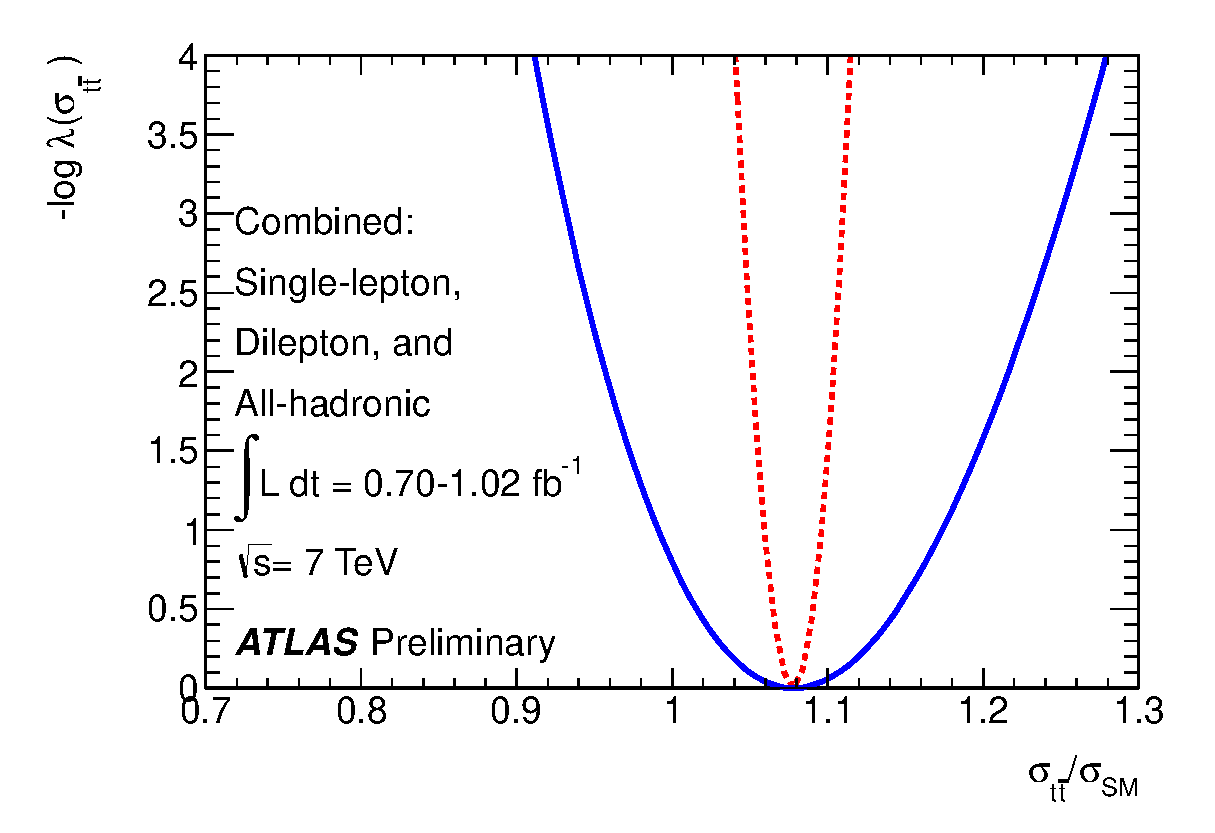
\includegraphics[width=.7\textwidth]{figures/comb/fullcombined_likelihood_curve}
    \caption{Graph of $-\log\lambda(\sigma_{\ttbar})$ vs. $\sigma_{\ttbar}/\sigma_{\rm SM}$ with (blue, solid) and without (red, dashed) systematic uncertainties for the six-channel combined fit.}
    \label{fig:fullcombined_likelihood_curve}
  \end{center}
\end{figure}
